\chapter{Requirements}

\section{Use-Case Diagram}
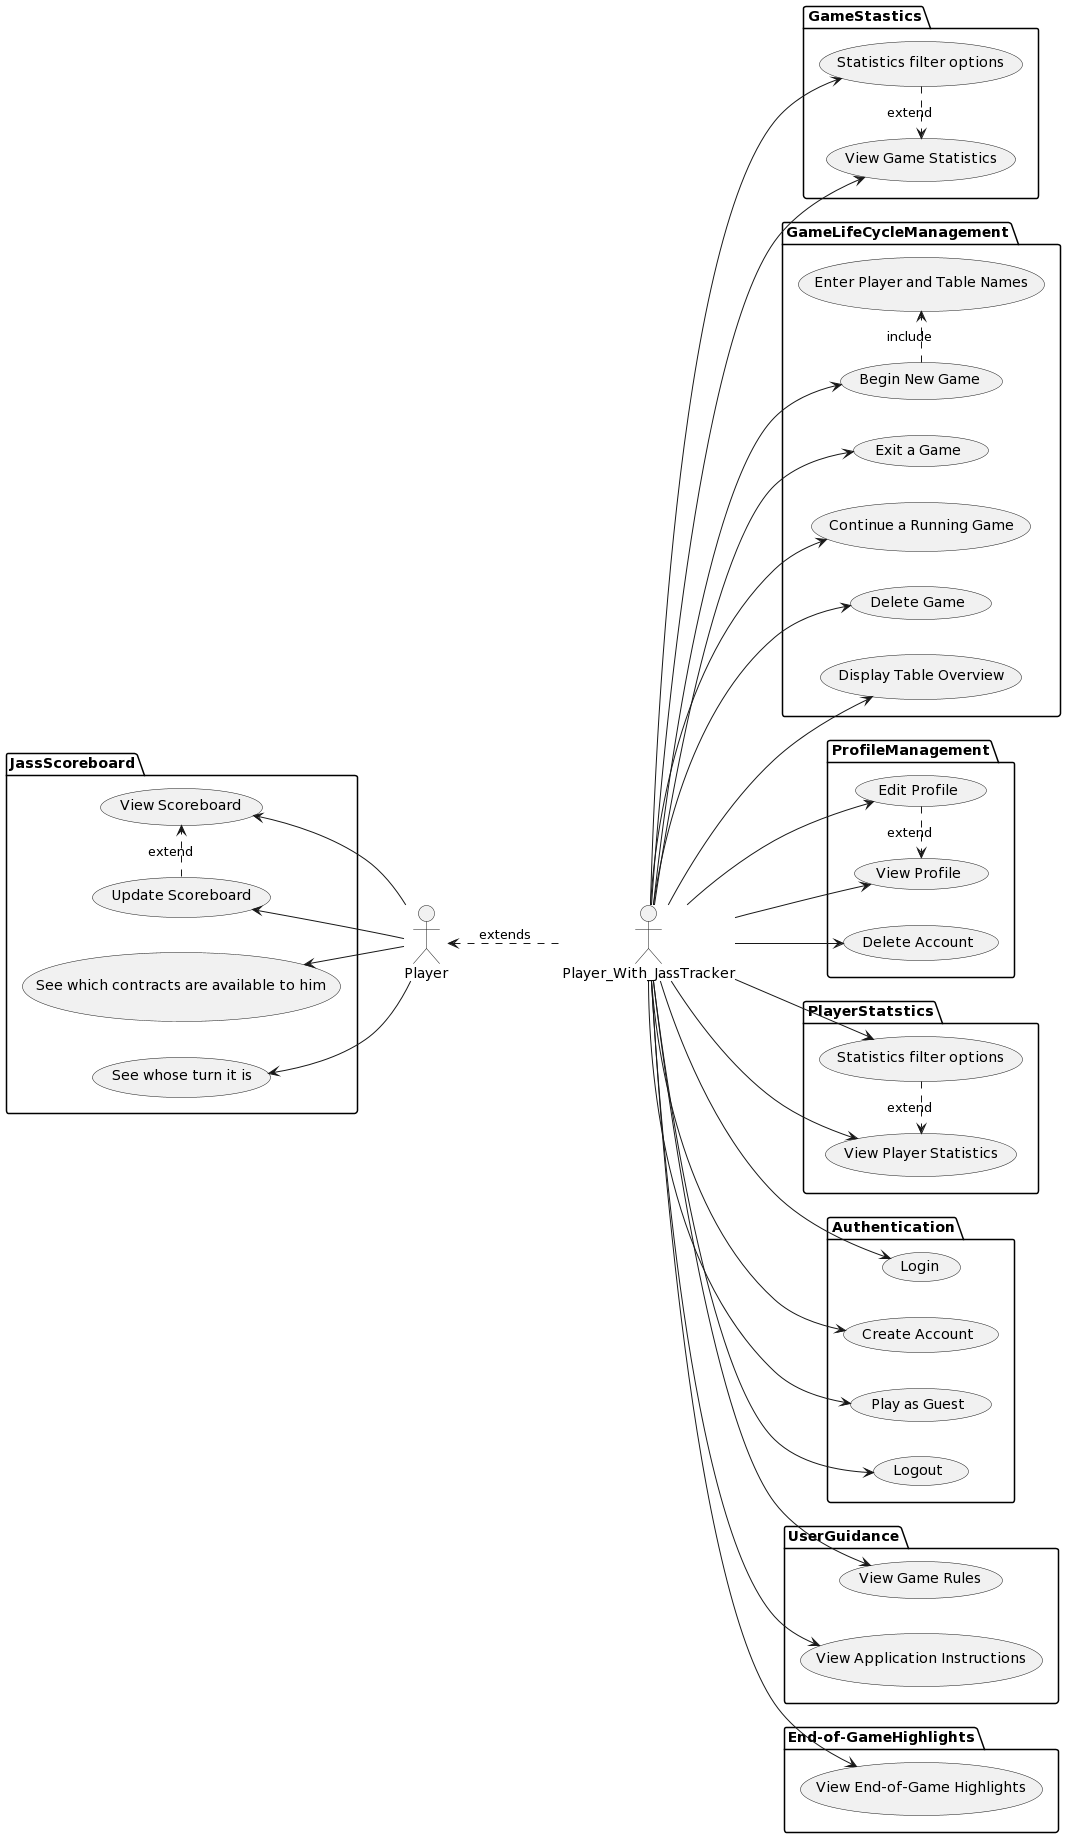
\includegraphics[height=18cm]{resources/diagrams/use-case}

\newcolumntype{s}{>{\columncolor[HTML]{c2c2cc}} m{3cm}} 

\section {Functional Requirements}

\paragraph{Info:}
The following requirements are by no means complete, but cover all key-requirements to aid the enhancement of use-cases and UI mockups. 
Also note that these requirements are not prioritized.

\subsection {Game Life Cycle Management}

\begin{tabular} { | m{1.75 cm} | m{5.25cm} | }
    \hline
    \multicolumn{1}{|c|}{\textbf{ID}} & \multicolumn{1}{|c|}{ \textbf{Story} }  \\
    \hline
    \href{https://jasstracker-jira.atlassian.net/browse/JASS-39}{JASS-39}  & New Table \& New Game Creation \\
    \hline
    \href{https://jasstracker-jira.atlassian.net/browse/JASS-43}{JASS-43} & Exit Game \\
    \hline
    \href{https://jasstracker-jira.atlassian.net/browse/JASS-41}{JASS-41} & Display Table Overview \\ 
    \hline
    \href{https://jasstracker-jira.atlassian.net/browse/JASS-42}{JASS-42} & Running \& Completed Game Distinction \\
    \hline
    \href{https://jasstracker-jira.atlassian.net/browse/JASS-41}{JASS-41} & Game Continuation \\ 
    \hline
    \href{https://jasstracker-jira.atlassian.net/browse/JASS-44}{JASS-44} & Delete Table \& Games \\
    \hline
\end{tabular}

\subsection{Jass Scoreboard}
\begin{tabular} { | m{1.75 cm} | m{5.25cm} | }
    \hline
    \multicolumn{1}{|c|}{\textbf{ID}} & \multicolumn{1}{|c|}{ \textbf{Story} }  \\
    \hline
    \href{https://jasstracker-jira.atlassian.net/browse/JASS-45}{JASS-45} & Display Current Score \\
    \hline
    \href{https://jasstracker-jira.atlassian.net/browse/JASS-46}{JASS-46} & Display Current Round \\
    \hline
    \href{https://jasstracker-jira.atlassian.net/browse/JASS-47}{JASS-47} & Enter Round Results \\
    \hline
    \href{https://jasstracker-jira.atlassian.net/browse/JASS-65}{JASS-65} & (Extension) View Win Probability per Team \\
    \hline
    \href{https://jasstracker-jira.atlassian.net/browse/JASS-64}{JASS-64} & (Extension) Display Score Prediction \\
    \hline
    \href{https://jasstracker-jira.atlassian.net/browse/JASS-66}{JASS-66} & (Extension) Share Scoreboard \\
    \hline
    \href{https://jasstracker-jira.atlassian.net/browse/JASS-48}{JASS-48} & Display Whose Turn it is \\
    \hline
    \href{https://jasstracker-jira.atlassian.net/browse/JASS-49}{JASS-49} & Display Teams \\
    \hline
\end{tabular}

\subsection{Game Statistics}
\begin{tabular} { | m{1.75 cm} | m{5.25cm} | }
    \hline
    \multicolumn{1}{|c|}{ \textbf{ID}} & \multicolumn{1}{|c|}{ \textbf{Story} }  \\
    \hline
    \href{https://jasstracker-jira.atlassian.net/browse/JASS-52}{JASS-52} & Display Statistics of one Game \\
    \hline
    \href{https://jasstracker-jira.atlassian.net/browse/JASS-53}{JASS-53} & (Extension) Display comparison of two game statistics \\
    \hline
    \href{https://jasstracker-jira.atlassian.net/browse/JASS-54}{JASS-54} & Display Statistics of one Round \\
    \hline
\end{tabular}

\subsection{User Account and Login}
\begin{tabular} { | m{1.75 cm} | m{5.25cm} | }
    \hline
    \multicolumn{1}{|c|}{ \textbf{ID}} & \multicolumn{1}{|c|}{ \textbf{Story} }  \\
    \hline
    \href{https://jasstracker-jira.atlassian.net/browse/JASS-51}{JASS-51} & Play as Guest \\
    \hline
    \href{https://jasstracker-jira.atlassian.net/browse/JASS-38}{JASS-38} & Account creation \\
    \hline
    \href{https://jasstracker-jira.atlassian.net/browse/JASS-37}{JASS-37} & Login \\
    \hline
    \href{https://jasstracker-jira.atlassian.net/browse/JASS-50}{JASS-50} & Logout \\
    \hline
\end{tabular}

\subsection{User Guidance}
\begin{tabular} { | m{1.75 cm} | m{5.25cm} | }
    \hline
    \multicolumn{1}{|c|}{ \textbf{ID}} & \multicolumn{1}{|c|}{ \textbf{Story} }  \\
    \hline
    \href{https://jasstracker-jira.atlassian.net/browse/JASS-36}{JASS-36} & Provide the rules of the game \\
    \hline
    \href{https://jasstracker-jira.atlassian.net/browse/JASS-56}{JASS-56} & Application Instructions \\
    \hline
\end{tabular}

\subsection{Profile Management}
\begin{tabular} { | m{1.75 cm} | m{5.25cm} | }
    \hline
    \multicolumn{1}{|c|}{ \textbf{ID}} & \multicolumn{1}{|c|}{ \textbf{Story} }  \\
    \hline
    \href{https://jasstracker-jira.atlassian.net/browse/JASS-33}{JASS-33} & Change Password \\
    \hline
    \href{https://jasstracker-jira.atlassian.net/browse/JASS-34}{JASS-34} & Account deletion \\
    \hline
    \href{https://jasstracker-jira.atlassian.net/browse/JASS-67}{JASS-67} & Add Displayname \\
    \hline
\end{tabular}

\subsection{Player Statistics}
\begin{tabular} { | m{1.75 cm} | m{5.25cm} | }
    \hline
    \multicolumn{1}{|c|}{ \textbf{ID}} & \multicolumn{1}{|c|}{ \textbf{Story} }  \\
    \hline
    \href{https://jasstracker-jira.atlassian.net/browse/JASS-32}{JASS-32} & Display unique player statistics \\
    \hline
\end{tabular}

\subsection{End-of-Game Highlights}
\begin{tabular} { | m{1.75 cm} | m{5.25cm} | }
    \hline
    \multicolumn{1}{|c|}{ \textbf{ID}} & \multicolumn{1}{|c|}{ \textbf{Story} } \\
    \hline
    \href{https://jasstracker-jira.atlassian.net/browse/JASS-68}{JASS-68} & End-of-Game Highlights \\
    \hline
\end{tabular}

\section {Non-Functional Requirements}

\renewcommand{\arraystretch}{1.5}

\subsection{Performance}
\begin{tabular} { |s| m{10.5cm } | }
    \hline
    \textbf{ID} & NFR-1 \\
    \hline
    \textbf{Requirement} & Reasonable response time for the rendering of new scores \\
    \hline
    \textbf{Trigger(s)} & User doesn't want to wait to see scores \\
    \hline
    \textbf{Measure(s)} & Rendering of the new scores must be doable within 1 second\\
    \hline
    \textbf{Testing} & Manual\\
    \hline
\end{tabular}
\newline
\vspace*{0.5 cm}
\newline
\begin{tabular} { |s|m{10.5cm} | }
    \hline
    \textbf{ID} & NFR-2 \\
    \hline
    \textbf{Requirement} & Authentication Response Time\\
    \hline
    \textbf{Trigger(s)} & User wants to be able to login in a timely manner\\
    \hline
    \textbf{Measure(s)} & Authentication of a user at login must be doable within 1 second\\
    \hline
    \textbf{Testing} & Manual\\
    \hline
\end{tabular}
\newline
\vspace*{0.5 cm}
\newline
\begin{tabular} { |s|m{10.5cm} | }
    \hline
    \textbf{ID} & NFR-3 \\
    \hline
    \textbf{Requirement} & New Game Creation Time\\
    \hline
    \textbf{Trigger(s)} & User wants to start the game as soon as possible\\
    \hline
    \textbf{Measure(s)} & Setting up a new game must be doable within 1 second\\
    \hline
    \textbf{Testing} & Manual\\
    \hline
\end{tabular}

\subsection{Usability}
\begin{tabular} { |s|m{10.5cm} | }
    \hline
    \textbf{ID} & NFR-4 \\
    \hline
    \textbf{Requirement} & Keyboard-only usability\\
    \hline
    \textbf{Trigger(s)} & User has no touch-screen or pointing device available\\ 
    \hline
    \textbf{Measure(s)} & Application must be usable with only a keyboard \\
    \hline
    \textbf{Testing} & Manual\\
    \hline
\end{tabular}
\newline
\vspace*{0.5 cm}
\newline
\begin{tabular} { |s|m{10.5cm} | }
    \hline
    \textbf{ID} & NFR-5 \\
    \hline
    \textbf{Requirement} & General Usability\\
    \hline
    \textbf{Trigger(s)} & Users want to be able to use the application without getting stuck\\
    \hline
    \textbf{Measure(s)} & Hallway testing shows eight people used the app without getting stuck\\
    \hline
    \textbf{Testing} & Manual\\
    \hline
\end{tabular}
\newline
\vspace*{0.5 cm}
\newline
\begin{tabular} { |s|m{10.5cm} | }
    \hline
    \textbf{ID} & NFR-6 \\
    \hline
    \textbf{Requirement} & User Guidance\\
    \hline
    \textbf{Trigger(s)} & User wants to be able to access a Help-Center\\
    \hline
    \textbf{Measure(s)} & Hallway testing shows eight people find the Help-Center and say it's helpful\\
    \hline
    \textbf{Testing} & Manual\\
    \hline
\end{tabular}


\subsection{Compatibility}
\begin{tabular} { |s|m{10.5cm} | }
    \hline
    \textbf{ID} & NFR-7 \\
    \hline
    \textbf{Requirement} & Browser Support\\
    \hline
    \textbf{Trigger(s)} & User wants to use a specific browser\\
    \hline
    \textbf{Measure(s)} & Last 2 major version of any browser with more than 1\% usage (except IE 11) is supported\\
    \hline
    \textbf{Testing} & Manual\\
    \hline
\end{tabular}
\newline
\vspace*{0.5 cm}
\newline
\begin{tabular} { |s|m{10.5cm} | }
    \hline
    \textbf{ID} & NFR-8 \\
    \hline
    \textbf{Requirement} & Mobile Device Support\\
    \hline
    \textbf{Trigger(s)} & User wants to access application via a Phone\\
    \hline
    \textbf{Measure(s)} & The application must support being used on mobile devices\\
    \hline
    \textbf{Testing} & Manual\\
    \hline
\end{tabular}

\subsection{Capacity}
\begin{tabular} { |s|m{10.5cm} | }
    \hline
    \textbf{ID} & NFR-9 \\
    \hline
    \textbf{Requirement} & Multiple accounts can be created \\
    \hline
    \textbf{Trigger(s)} & More than one person wants to use the application not as a guest\\
    \hline
    \textbf{Measure(s)} & At least 500 users can create an account\\
    \hline
    \textbf{Testing} & Automated\\
    \hline
\end{tabular}
\newline
\vspace*{0.5 cm}
\newline
\begin{tabular} { |s|m{10.5cm} | }
    \hline
    \textbf{ID} & NFR-10 \\
    \hline
    \textbf{Requirement} & Multiple games can be running at one time\\
    \hline
    \textbf{Trigger(s)} & A user is active in more than one game\\
    \hline
    \textbf{Measure(s)} & At least 4 games can be running at one time for a single user \\
    \hline
    \textbf{Testing} & Automated\\
    \hline
\end{tabular}

\subsection{Availability}
\begin{tabular} { |s|m{10.5cm} | }
    \hline
    \textbf{ID} & NFR-11 \\
    \hline
    \textbf{Requirement} & The application must be available \\
    \hline
    \textbf{Trigger(s)} & Application crash\\
    \hline
    \textbf{Measure(s)} & Average downtime can not exceed 30 minutes per day\\
    \hline
    \textbf{Testing} & Automated\\
    \hline
\end{tabular}

\subsection{Recoverability}
\begin{tabular} { |s|m{10.5cm} | }
    \hline
    \textbf{ID} & NFR-12 \\
    \hline
    \textbf{Requirement} & The application must not lose state \\
    \hline
    \textbf{Trigger(s)} & Application crash\\
    \hline
    \textbf{Measure(s)} & The state before crash must be recoverable\\
    \hline
    \textbf{Testing} & Automated\\
    \hline
\end{tabular}

\subsection{Maintainability}
\begin{tabular} { |s|m{10.5cm} | }
    \hline
    \textbf{ID} & NFR-13 \\
    \hline
    \textbf{Requirement} & Code Base Understanding\\
    \hline
    \textbf{Trigger(s)} & Any developer wants to be able to understand the code base\\
    \hline
    \textbf{Measure(s)} & SonarQube \\
    \hline
    \textbf{Testing} & Automated\\
    \hline
\end{tabular}
\newline
\vspace*{0.5 cm}
\newline
\begin{tabular} { |s|m{10.5cm} | }
    \hline
    \textbf{ID} & NFR-14 \\
    \hline
    \textbf{Requirement} & Test-Coverage\\
    \hline
    \textbf{Trigger(s)} & User wants accountability for business functionality\\
    \hline
    \textbf{Measure(s)} & At least 80\% test-coverage is required for business logic\\
    \hline
    \textbf{Testing} & Automated\\
    \hline
\end{tabular}
\newline
\vspace*{0.5 cm}
\newline
\begin{tabular} { |s|m{10.5cm} | }
    \hline
    \textbf{ID} & NFR-15 \\
    \hline
    \textbf{Requirement} & Logging\\
    \hline
    \textbf{Trigger(s)} & User action needs to be reviewed\\
    \hline
    \textbf{Measure(s)} & At least one human readable log statement is available for each user action\\
    \hline
    \textbf{Testing} & Manual\\
    \hline
\end{tabular}
\newline
\vspace*{0.5 cm}
\newline
\begin{tabular} { |s|m{10.5cm} | }
    \hline
    \textbf{ID} & NFR-16 \\
    \hline
    \textbf{Requirement} & Lighthouse categories are acceptable\\
    \hline
    \textbf{Trigger(s)} & Users want a fast and accessible app  \\
    \hline
    \textbf{Measure(s)} & Web app should pass performance, accessibility and best practices in lighthouse with a green color (90+)\\
    \hline
    \textbf{Testing} & Automated with Gitlab CI/CD\\
    \hline
\end{tabular}

\subsection{Security}
\begin{tabular} { |s|m{10.5cm} | }
    \hline
    \textbf{ID} & NFR-17 \\
    \hline
    \textbf{Requirement} & Passwords must be secure \\
    \hline
    \textbf{Trigger(s)} & A not safe (in length) password is created\\
    \hline
    \textbf{Measure(s)} & Passwords must be at least eight characters in length\\
    \hline
    \textbf{Testing} & Automated\\
    \hline
\end{tabular}

\pagebreak
\section {Mockups}

\paragraph{Disclaimer:}
These are just Mockups.
Design can still change and colours aren't fixed and are just as a visual aid for where containers should go.


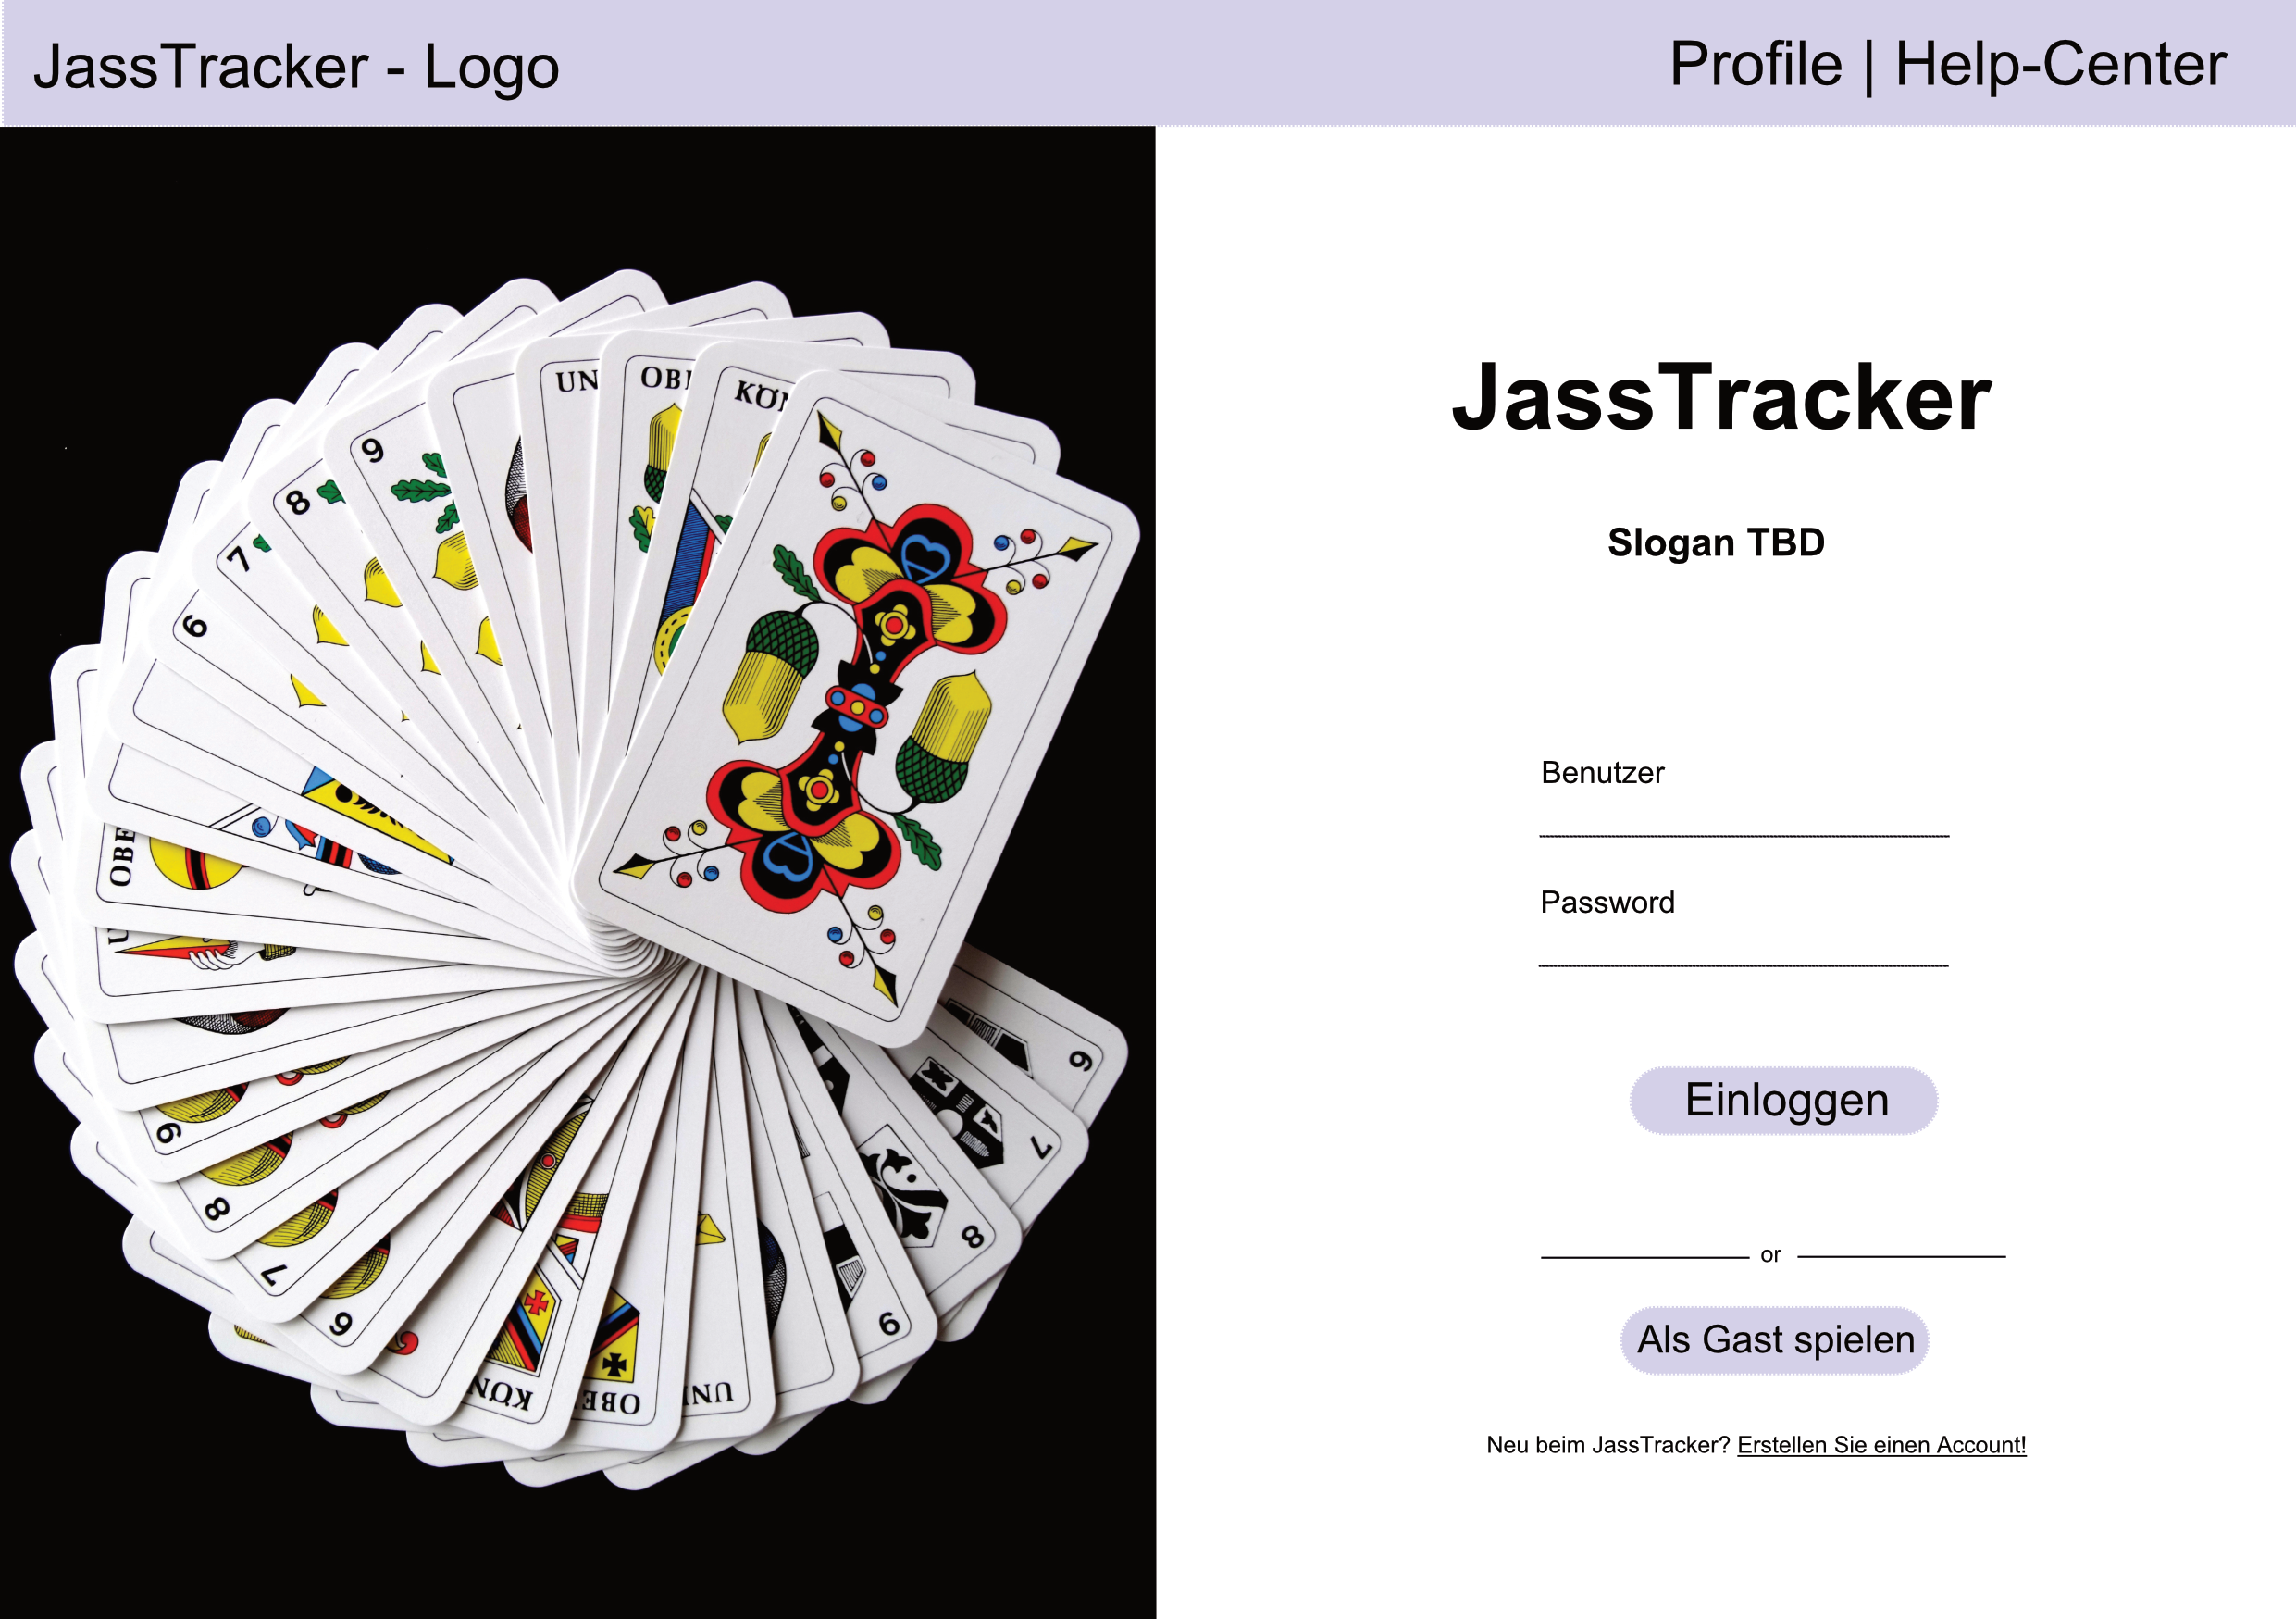
\includegraphics[height=10cm, width=\textwidth]{resources/mockups/mockup-login}
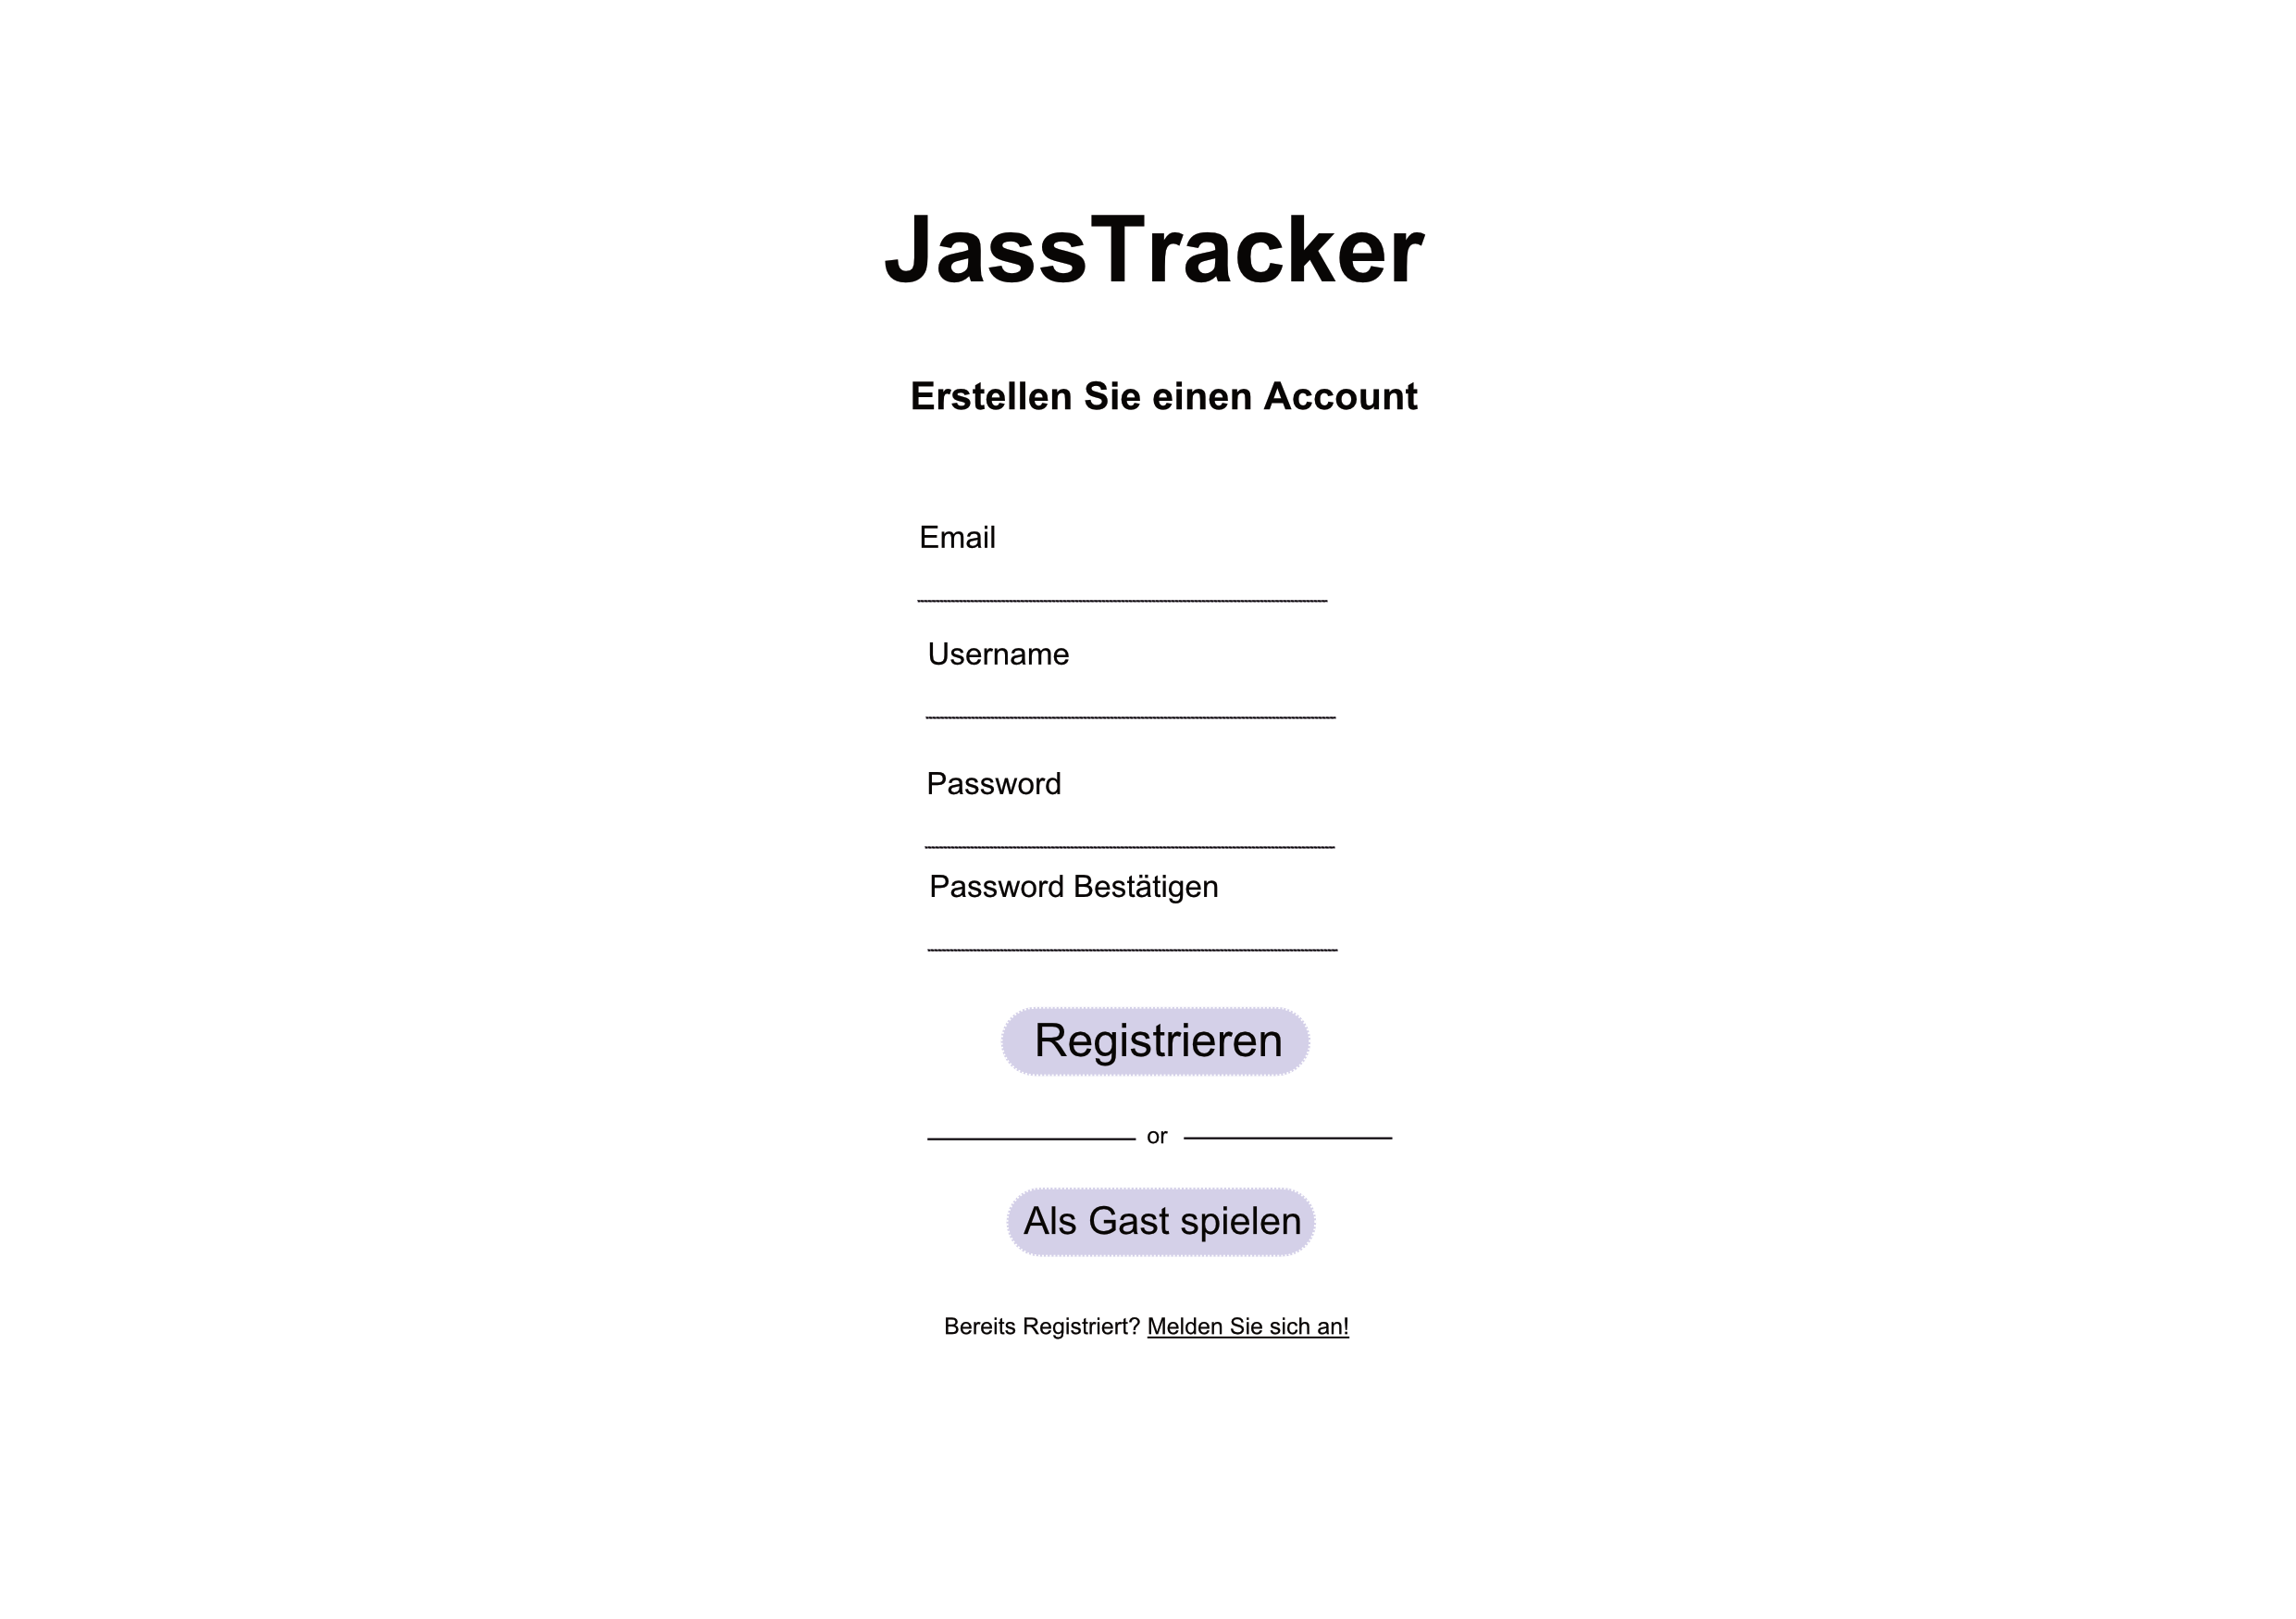
\includegraphics[height=10cm, width=\textwidth]{resources/mockups/mockup-register}
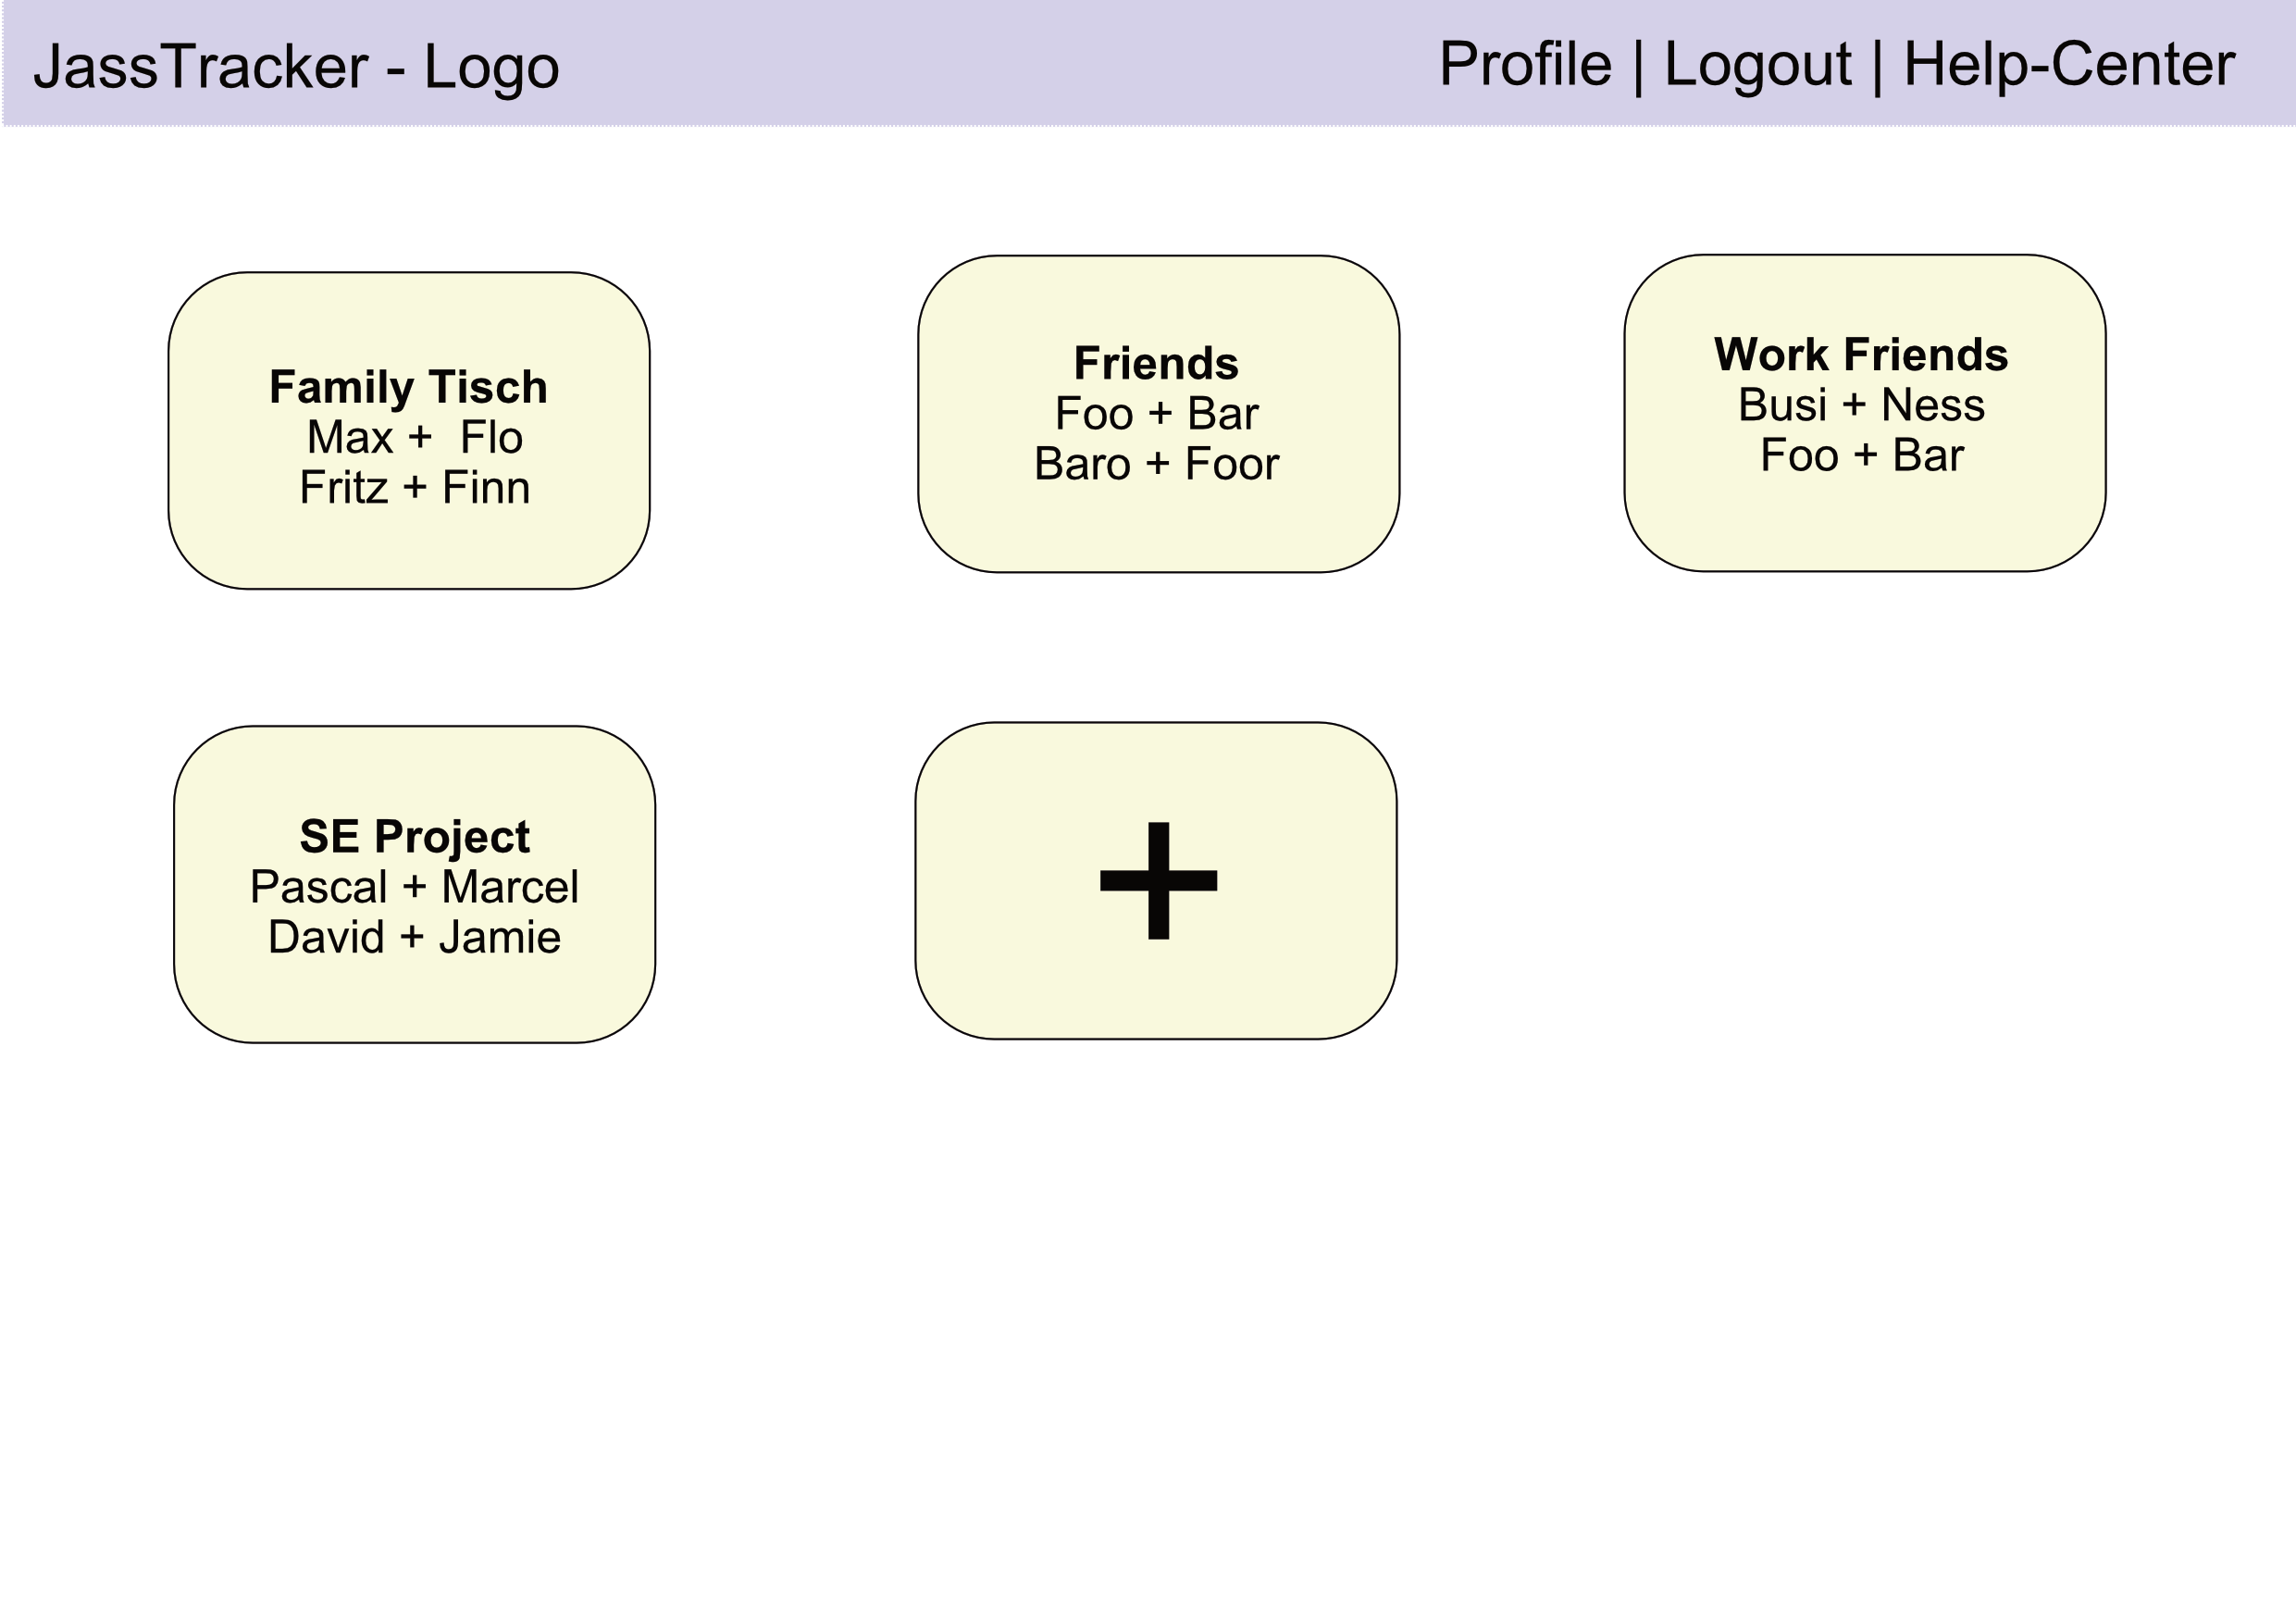
\includegraphics[height=10cm, width=\textwidth]{resources/mockups/mockup-table-overview}
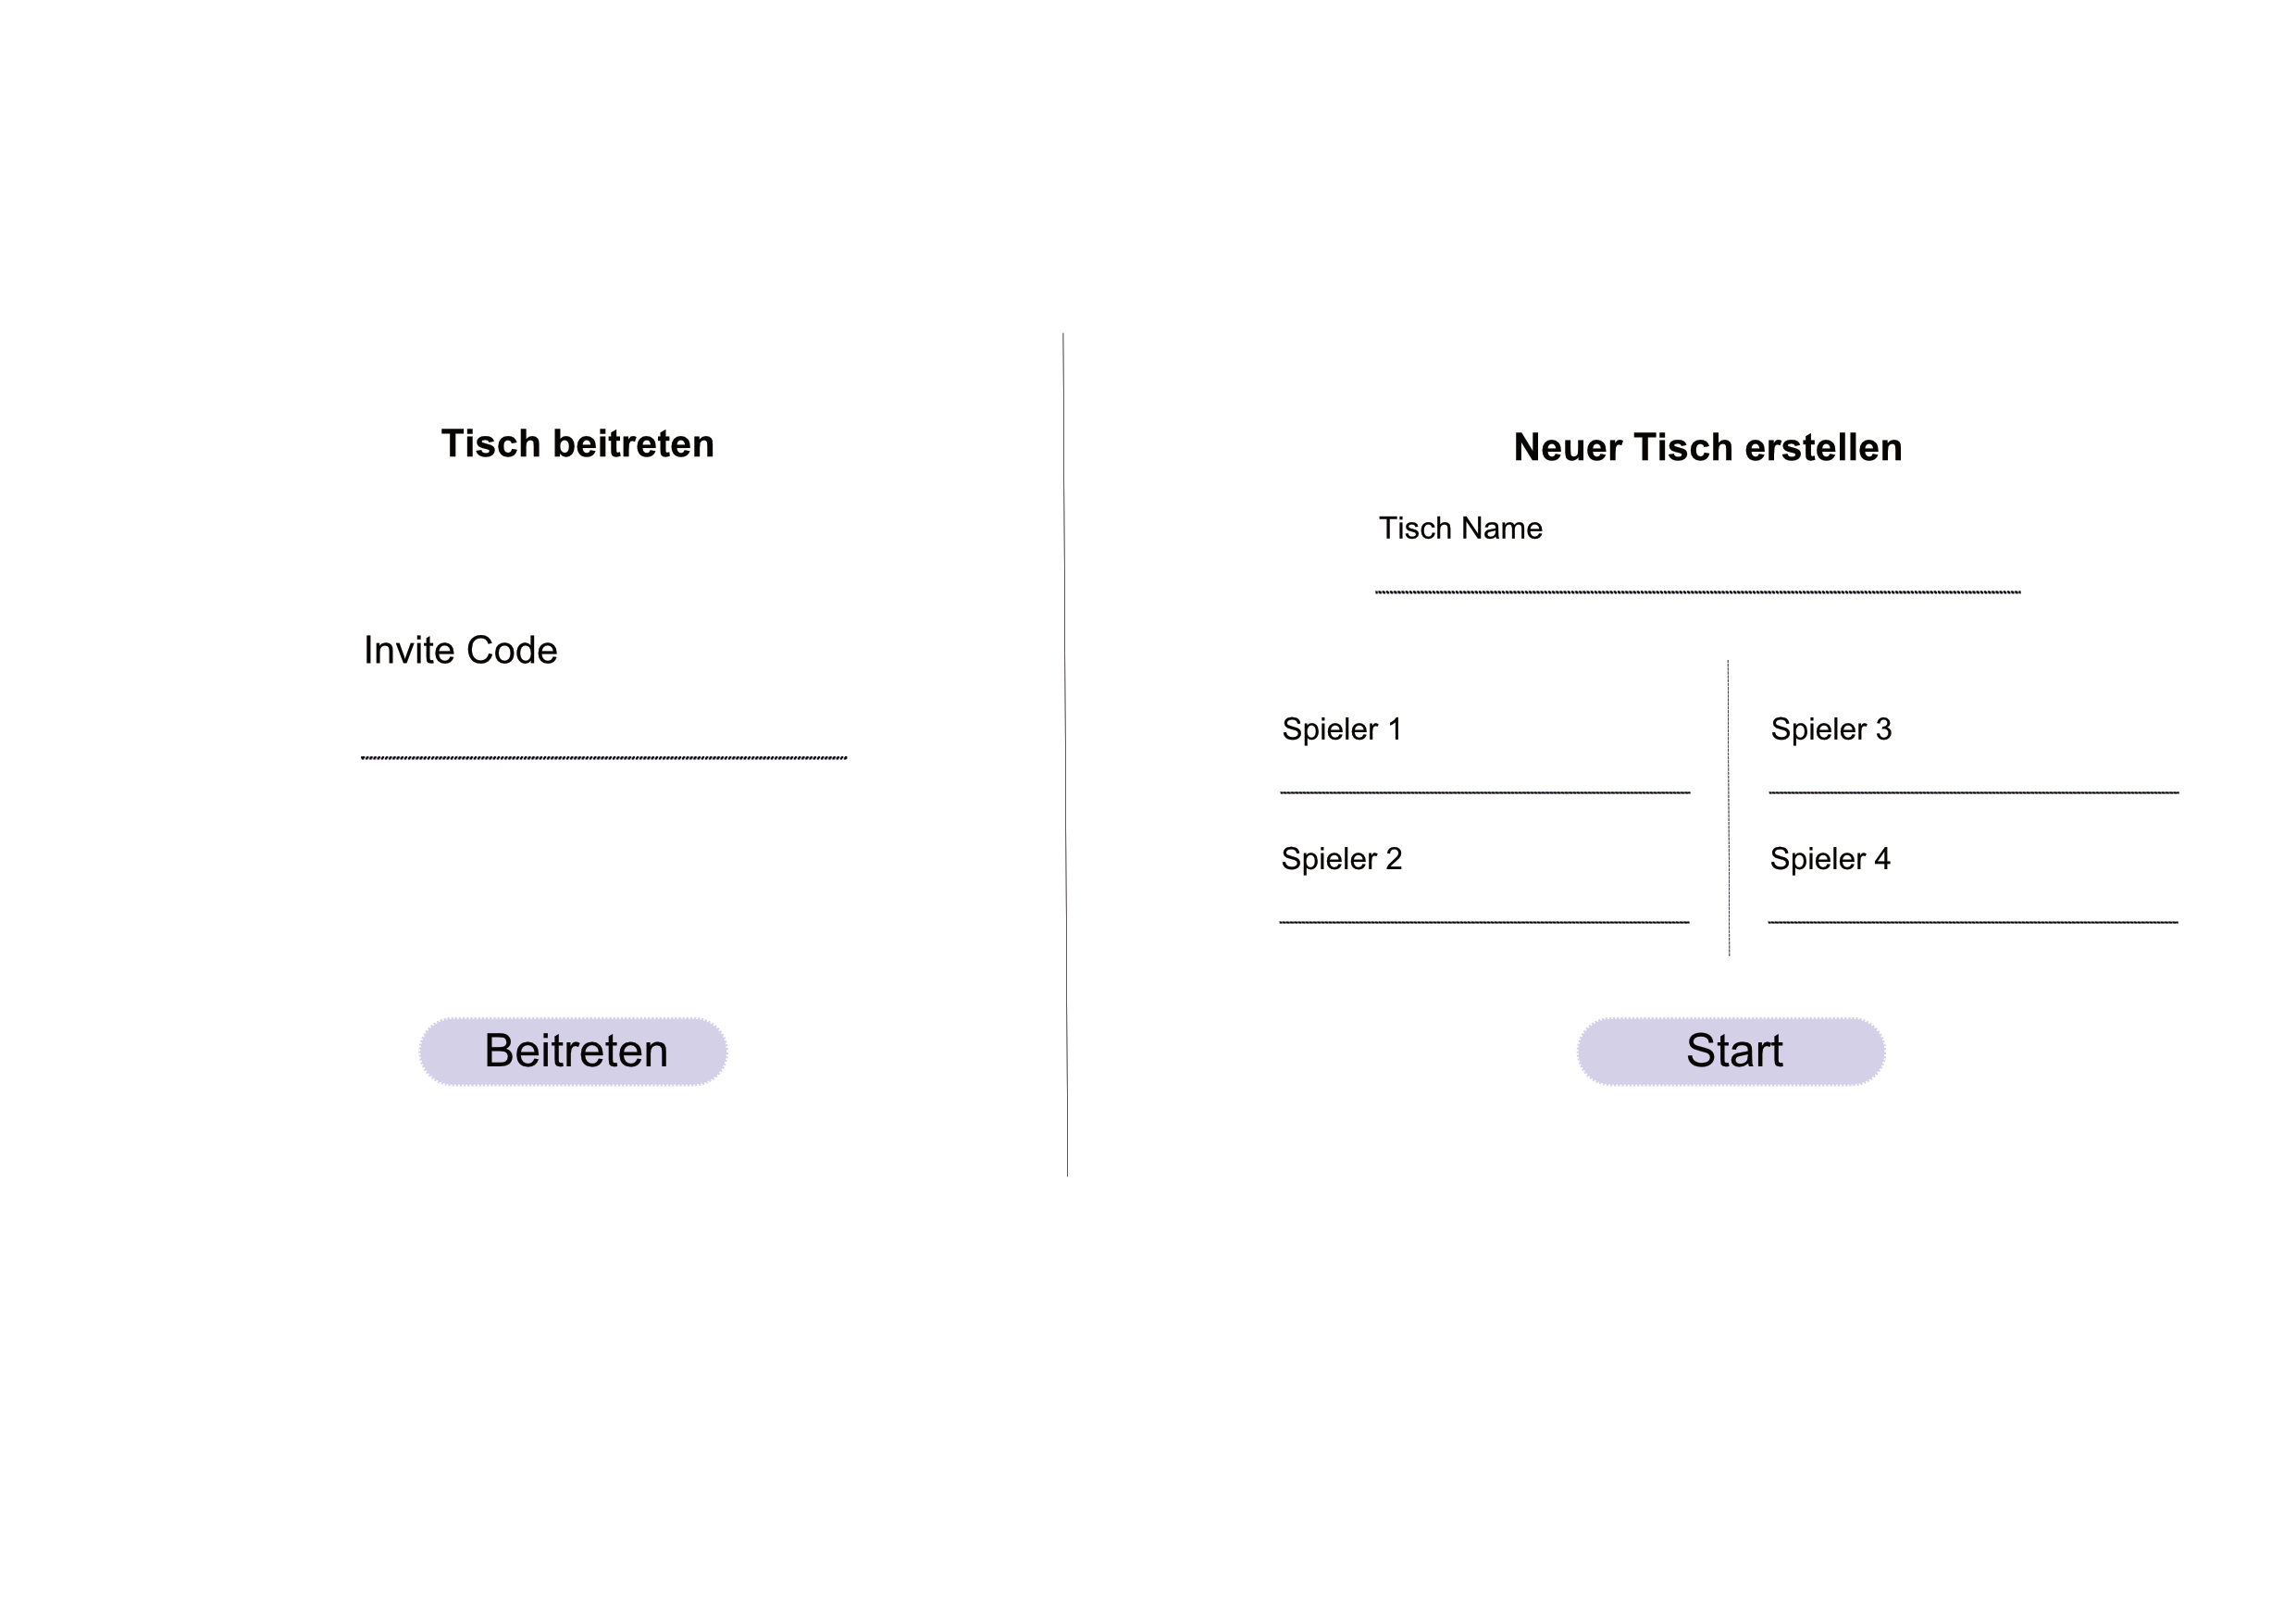
\includegraphics[height=10cm, width=\textwidth]{resources/mockups/mockup-create-new-table}
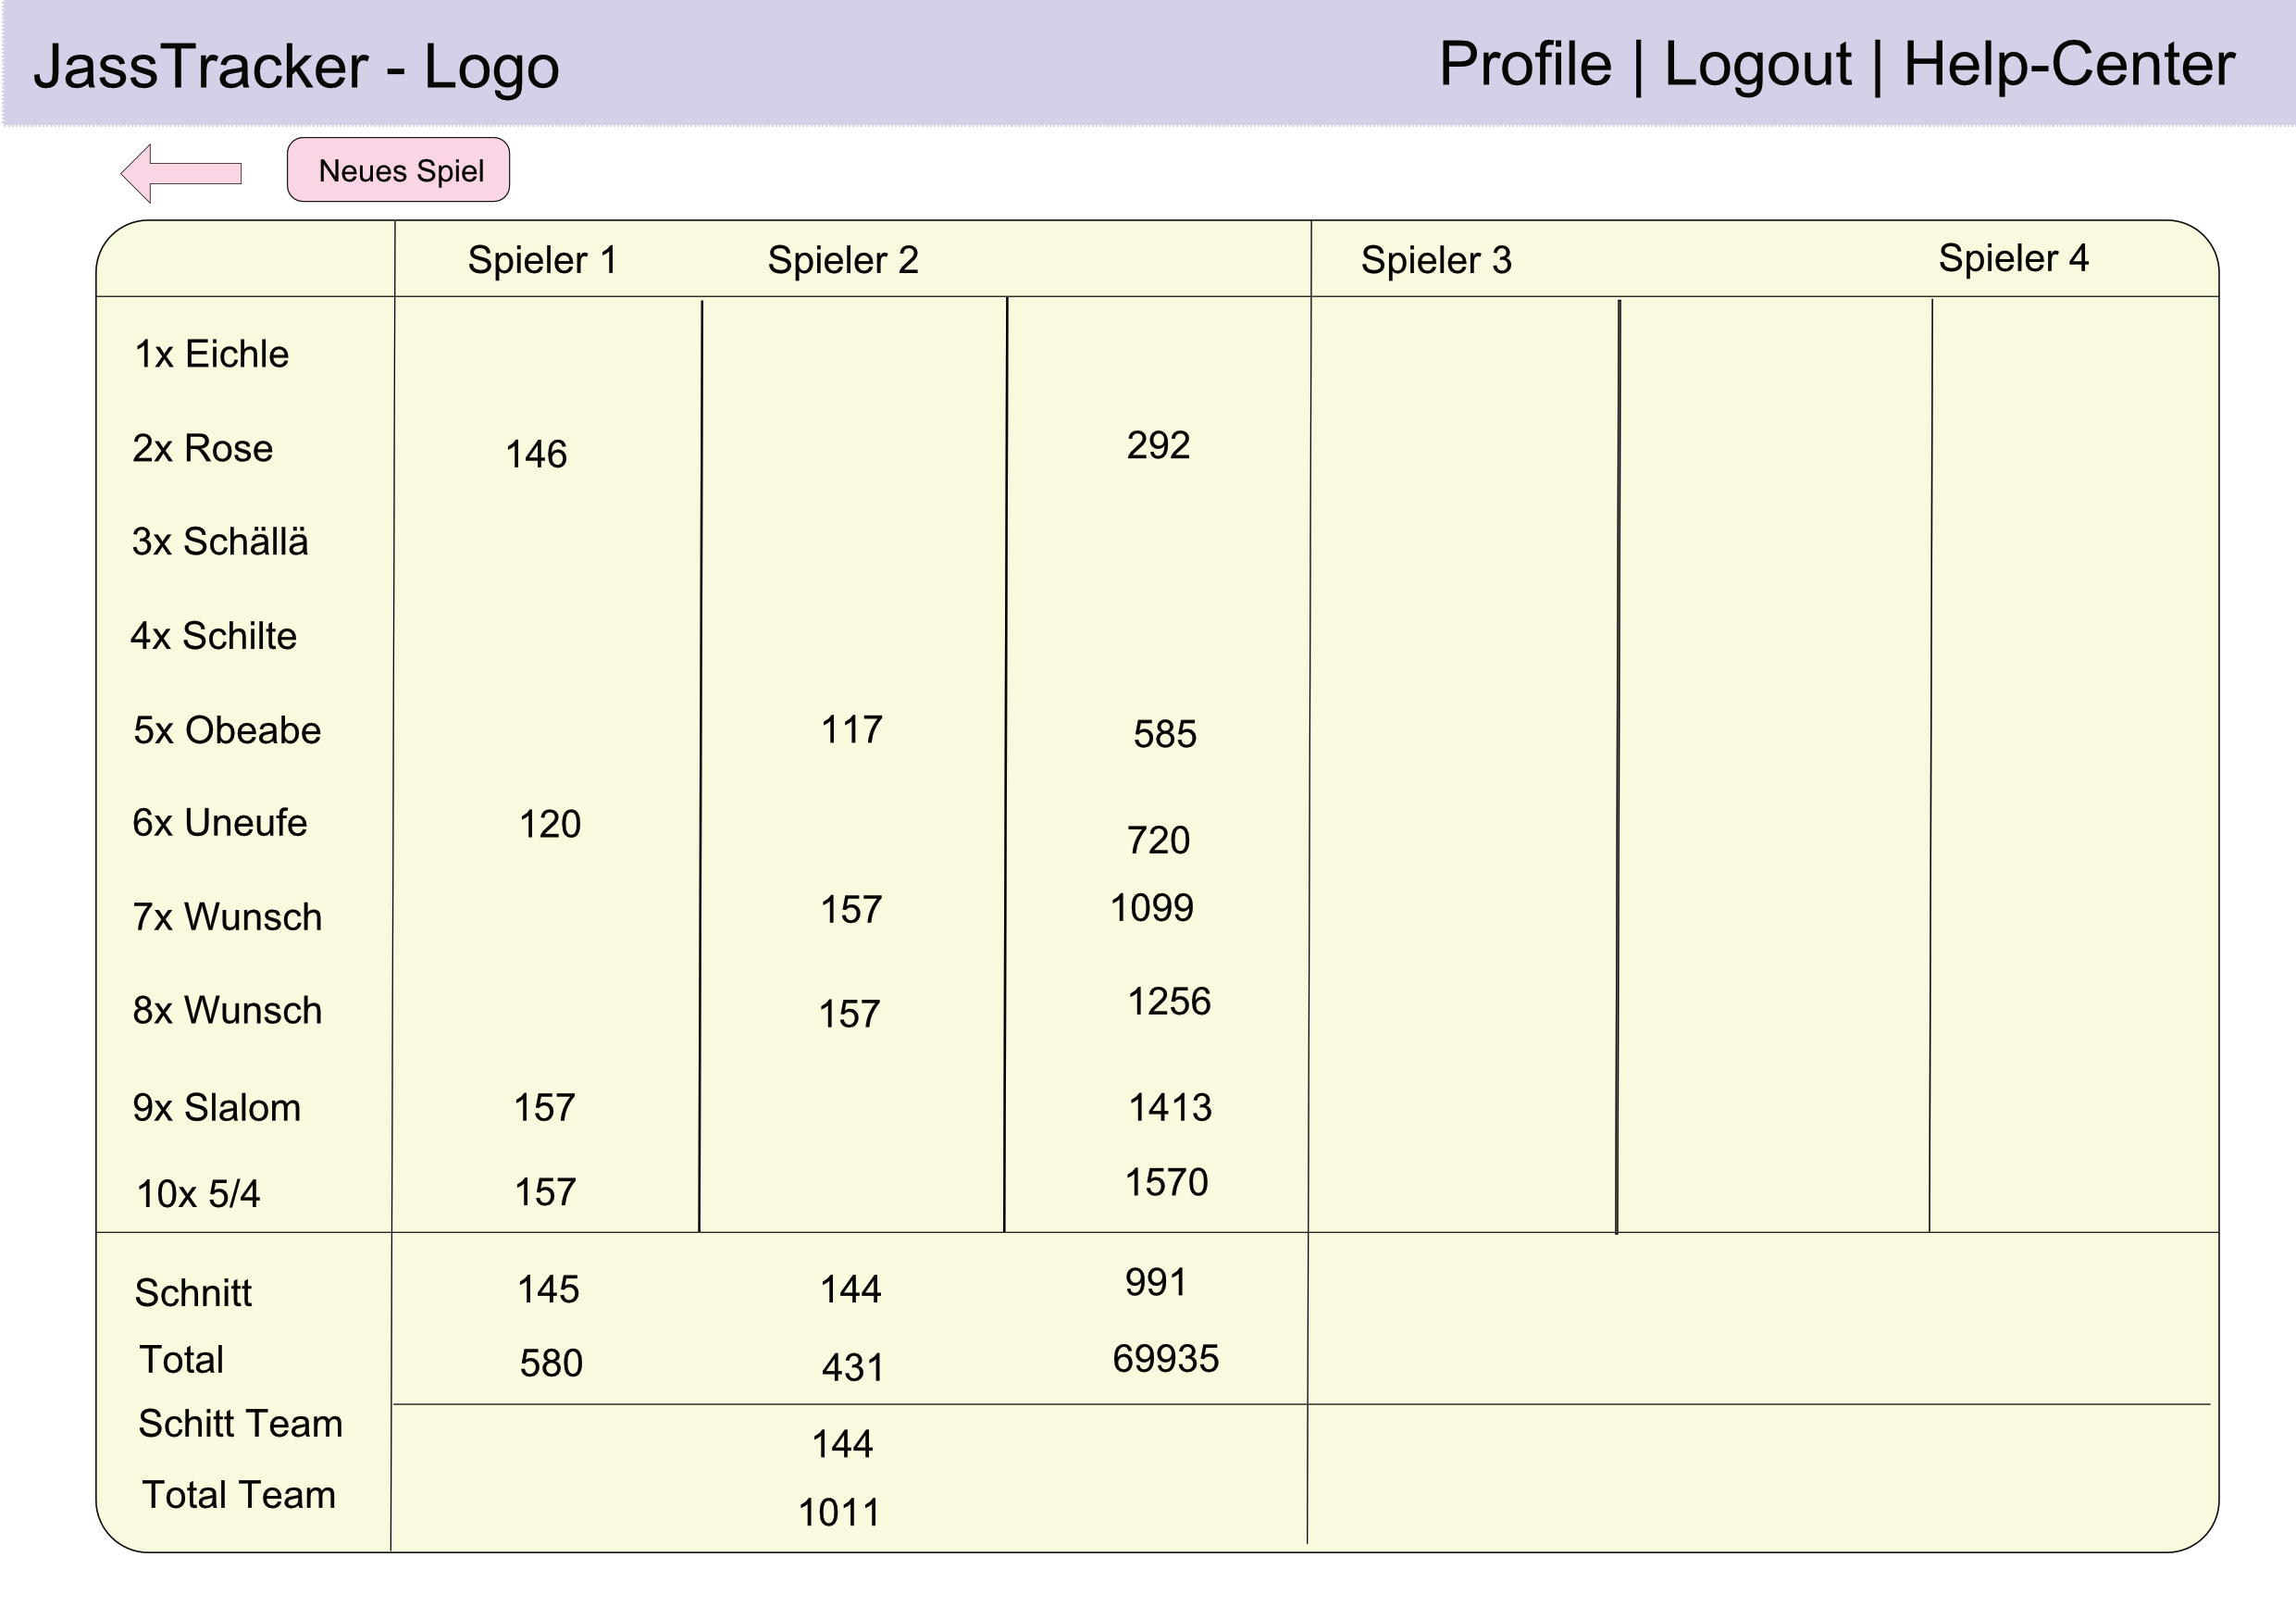
\includegraphics[height=10cm, width=\textwidth]{resources/mockups/mockup-scoreboard}
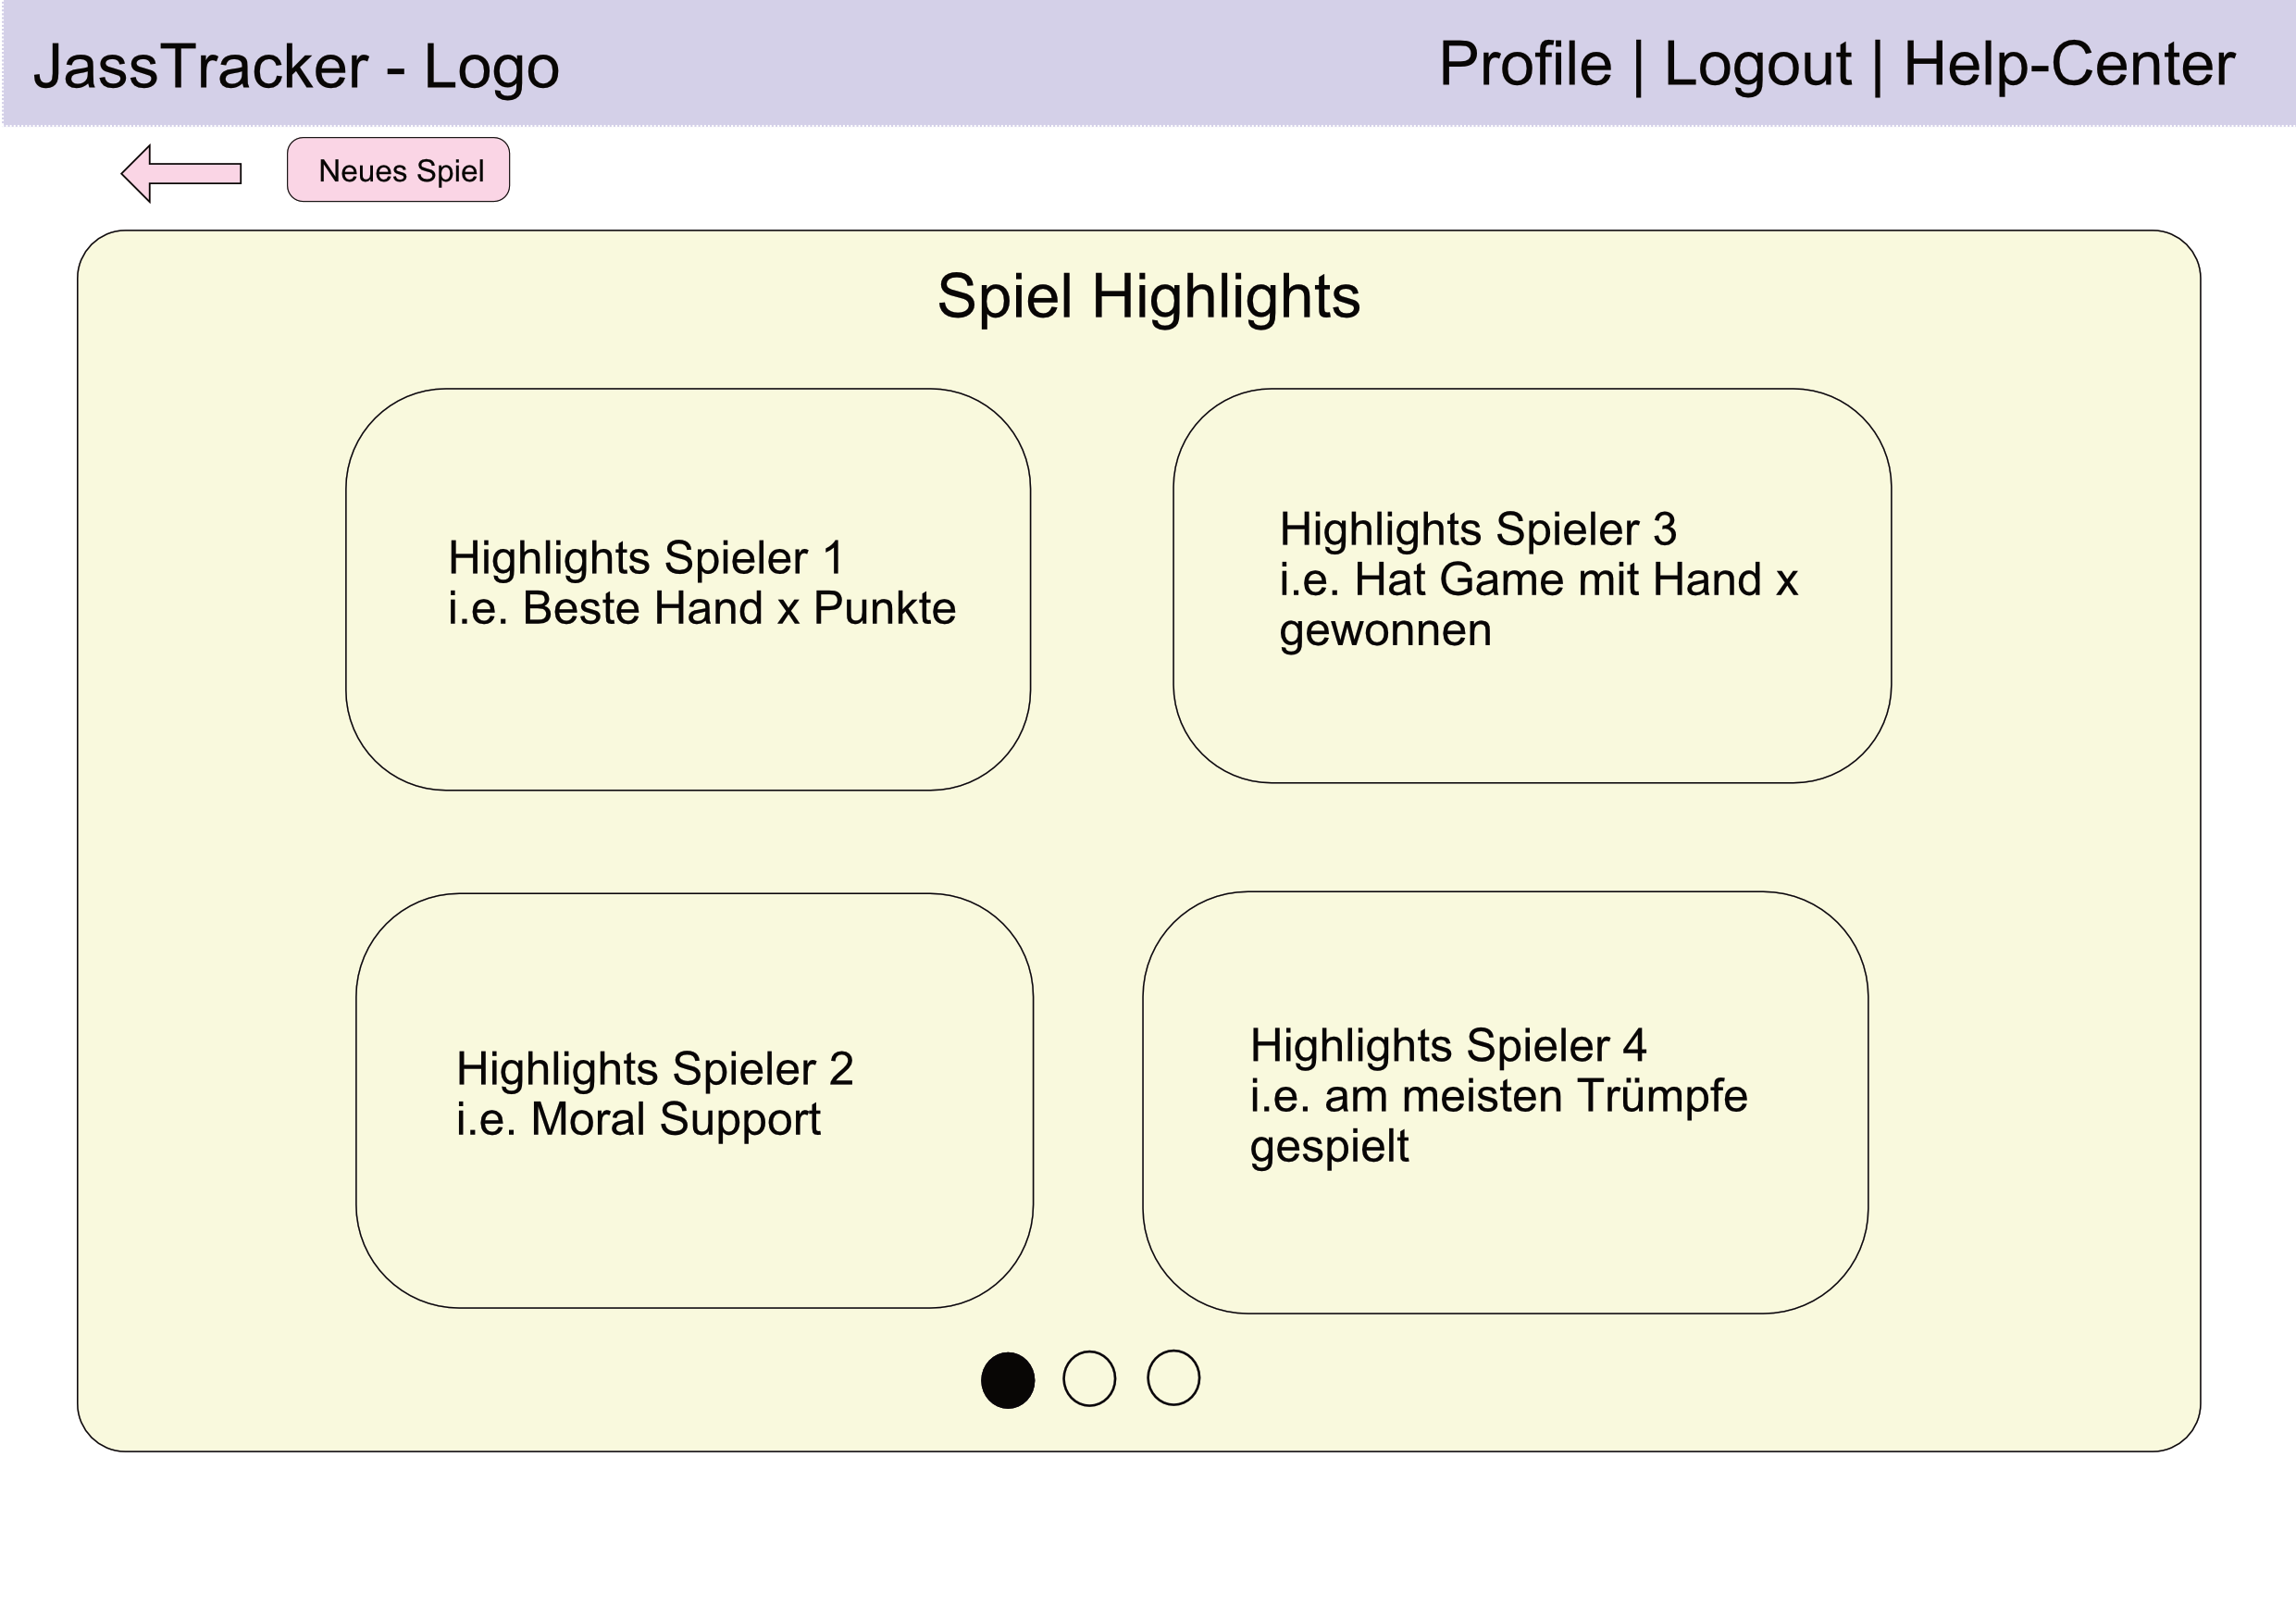
\includegraphics[height=10cm, width=\textwidth]{resources/mockups/mockup-eof-highlights}
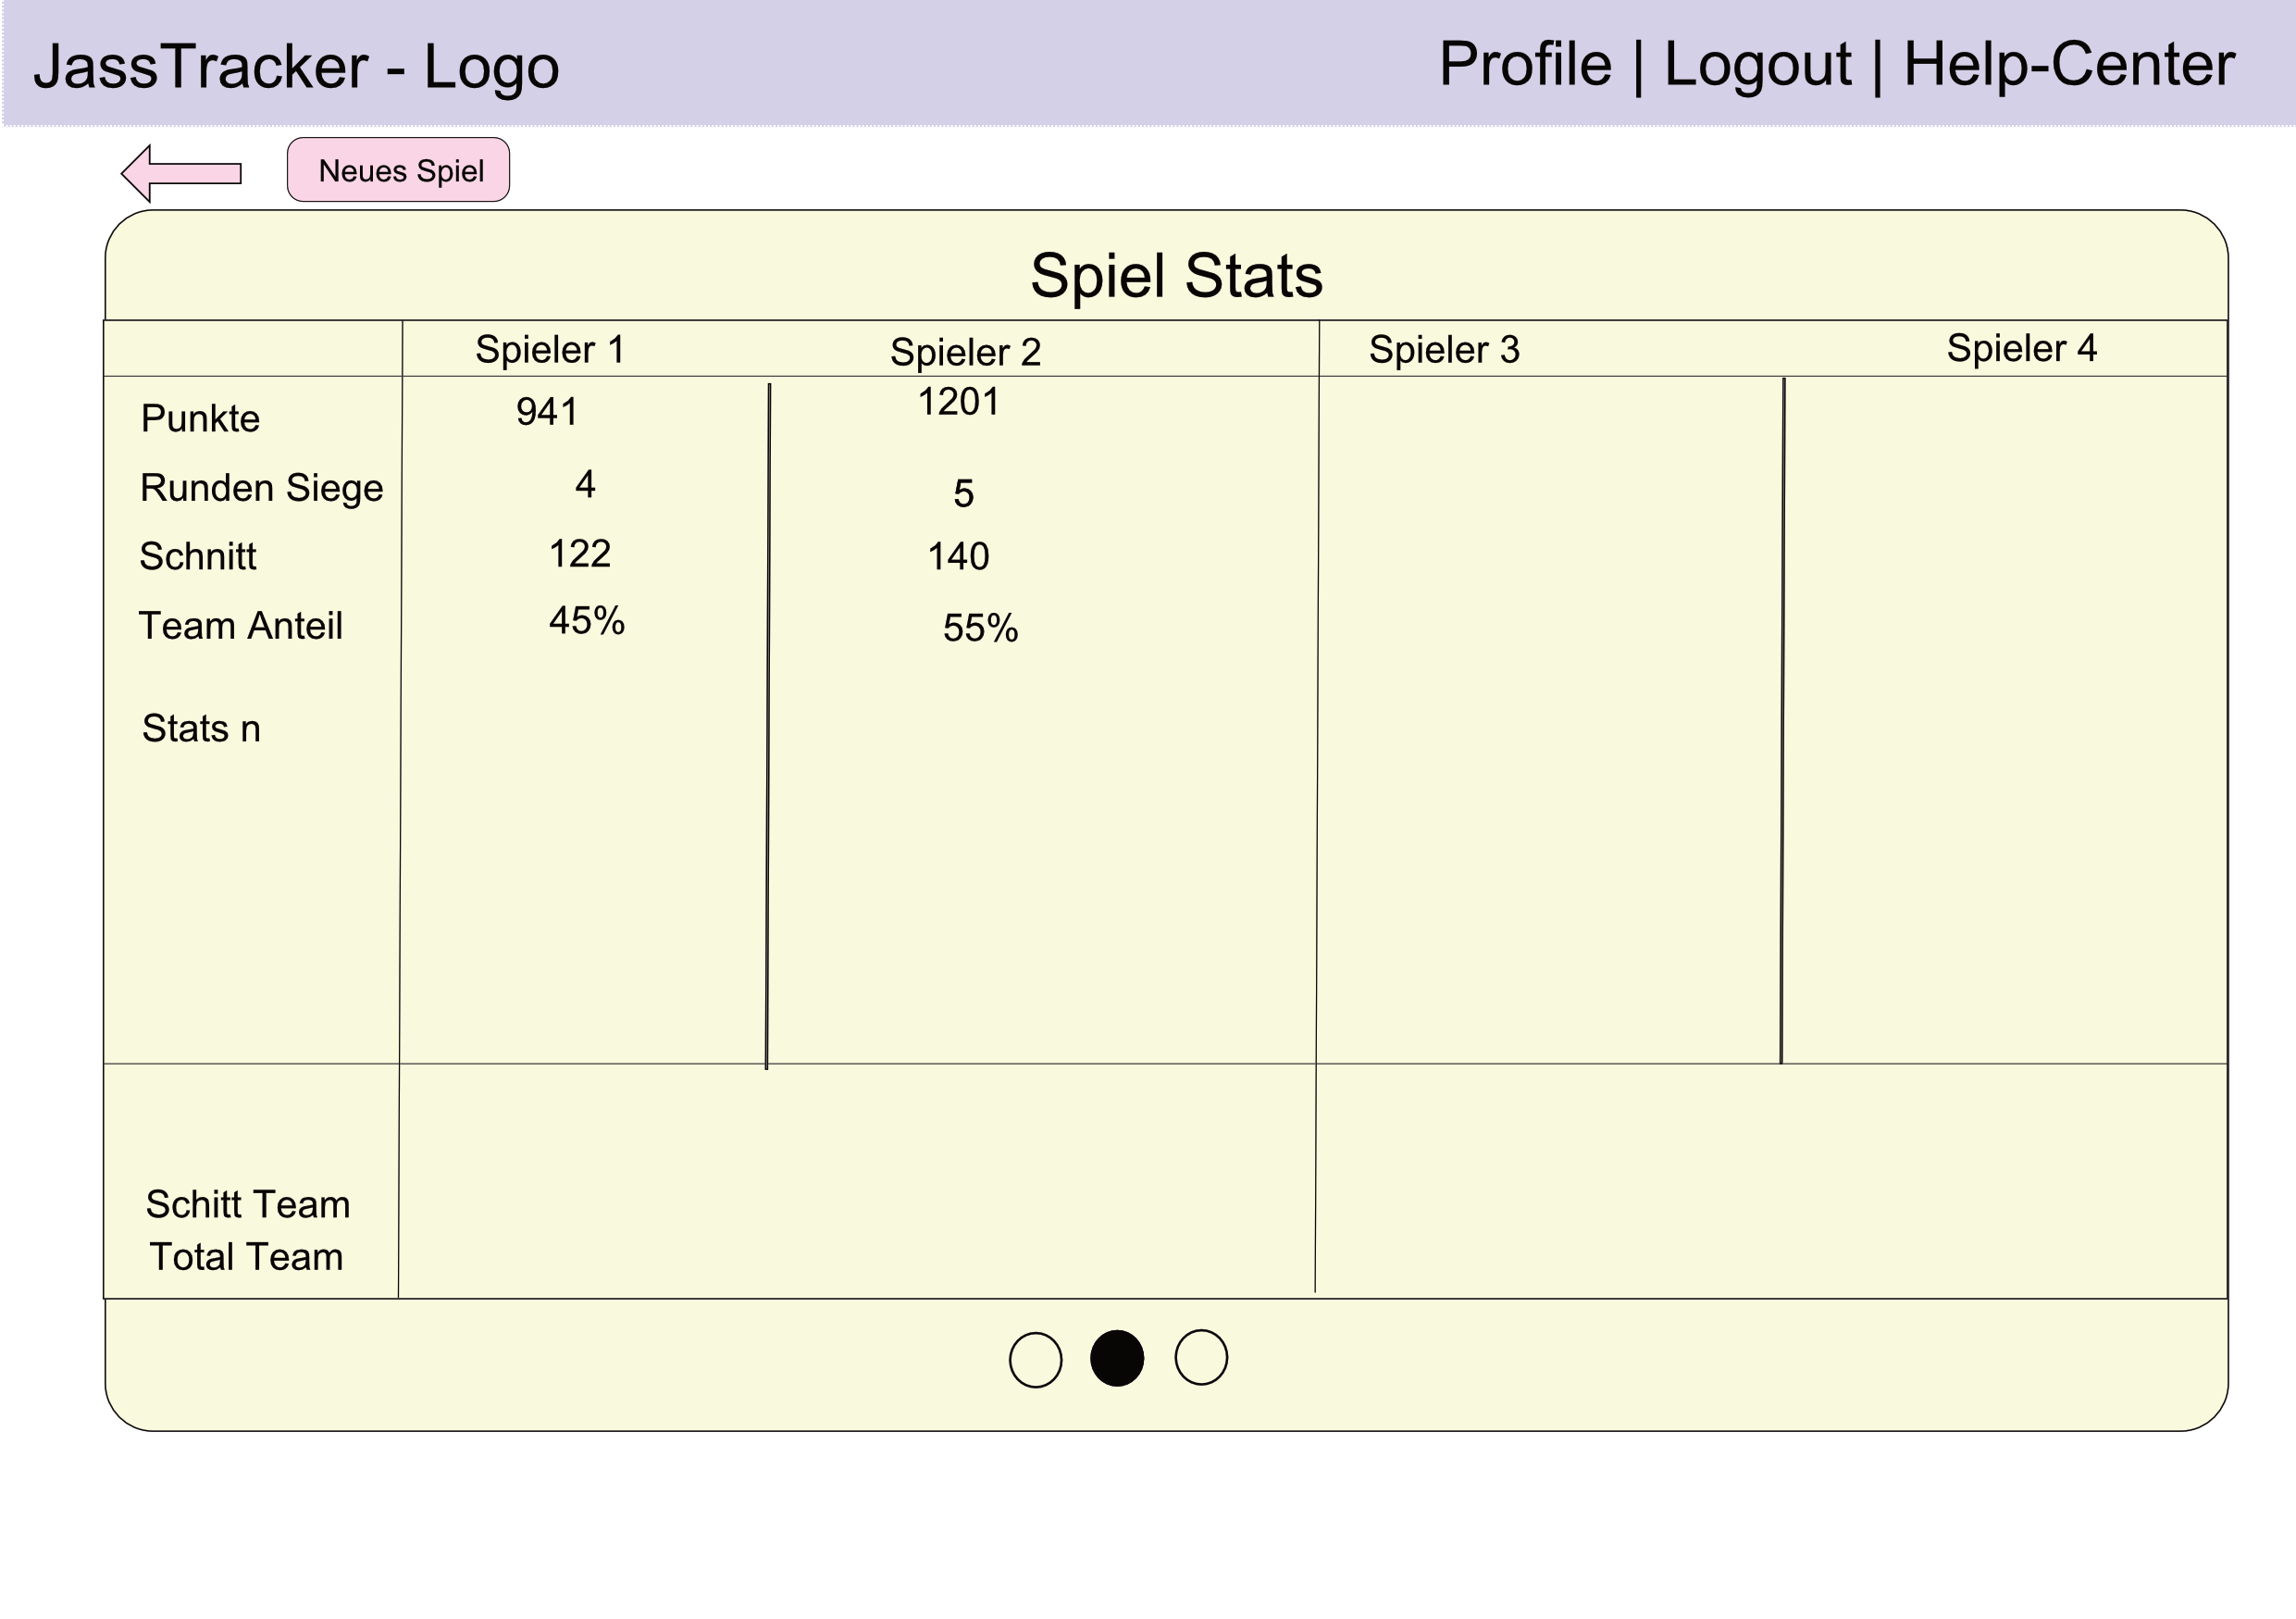
\includegraphics[height=10cm, width=\textwidth]{resources/mockups/mockup-eof-stats}
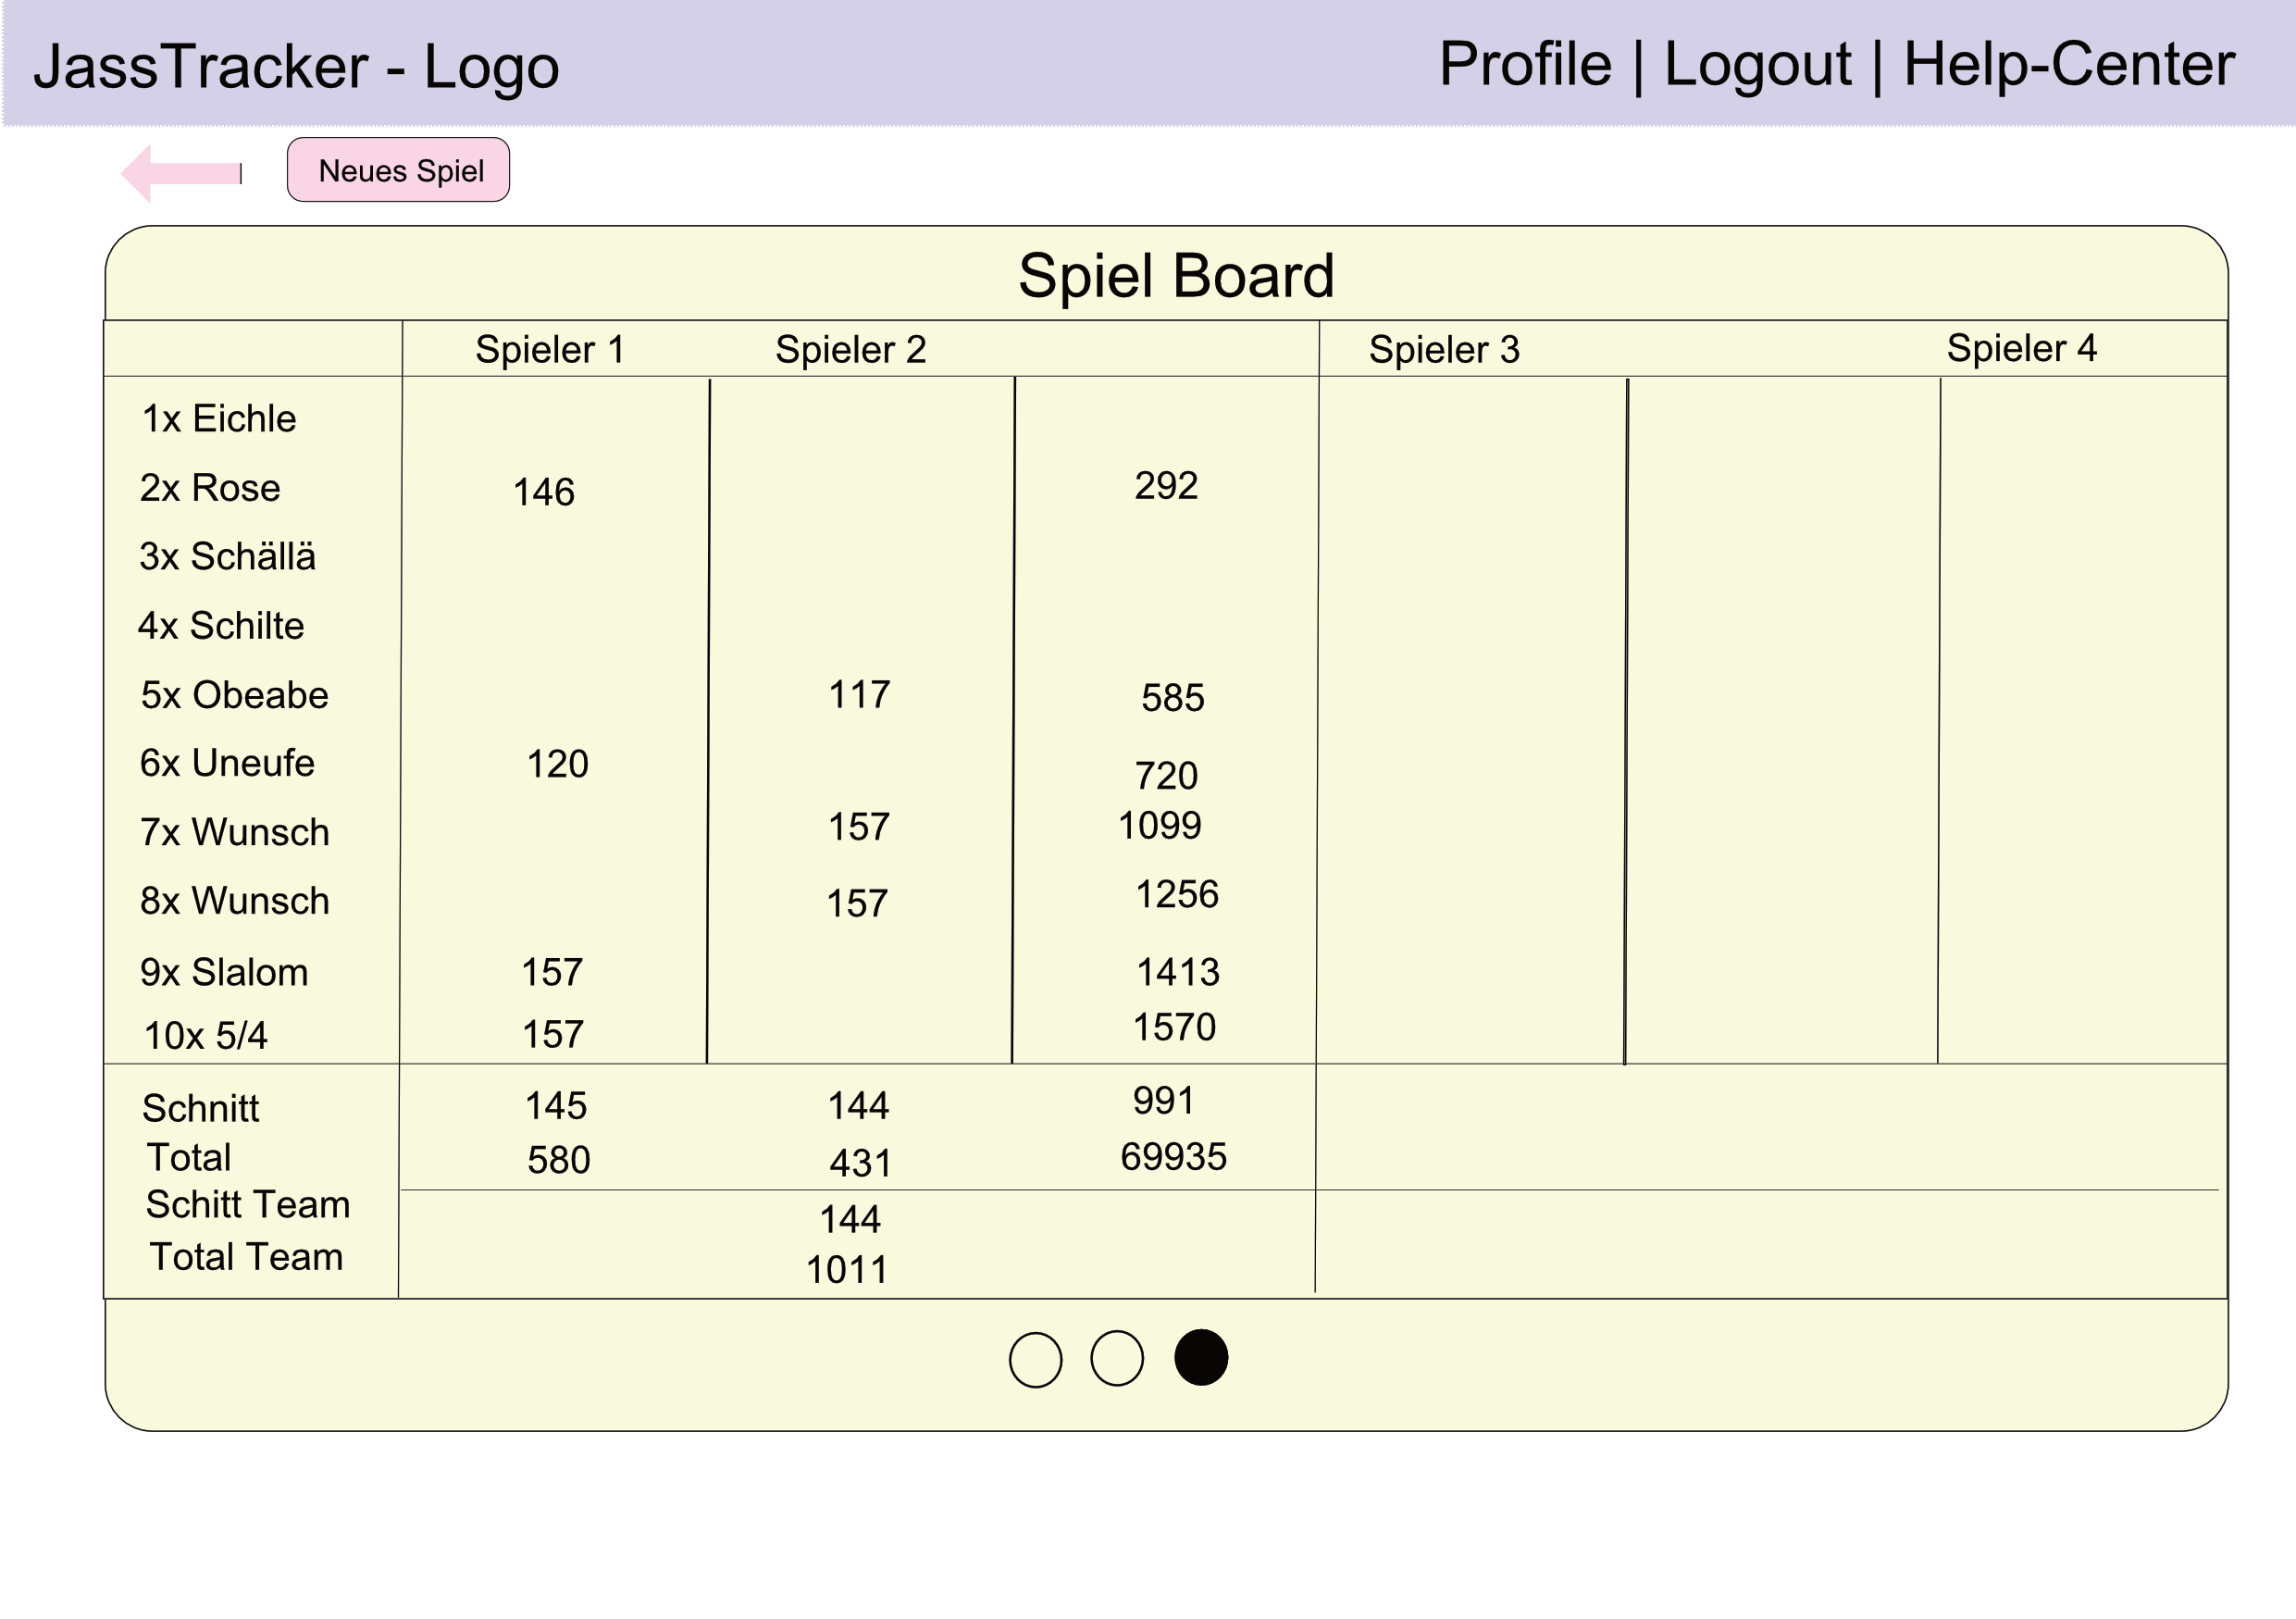
\includegraphics[height=10cm, width=\textwidth]{resources/mockups/mockup-eof-scoreboard}
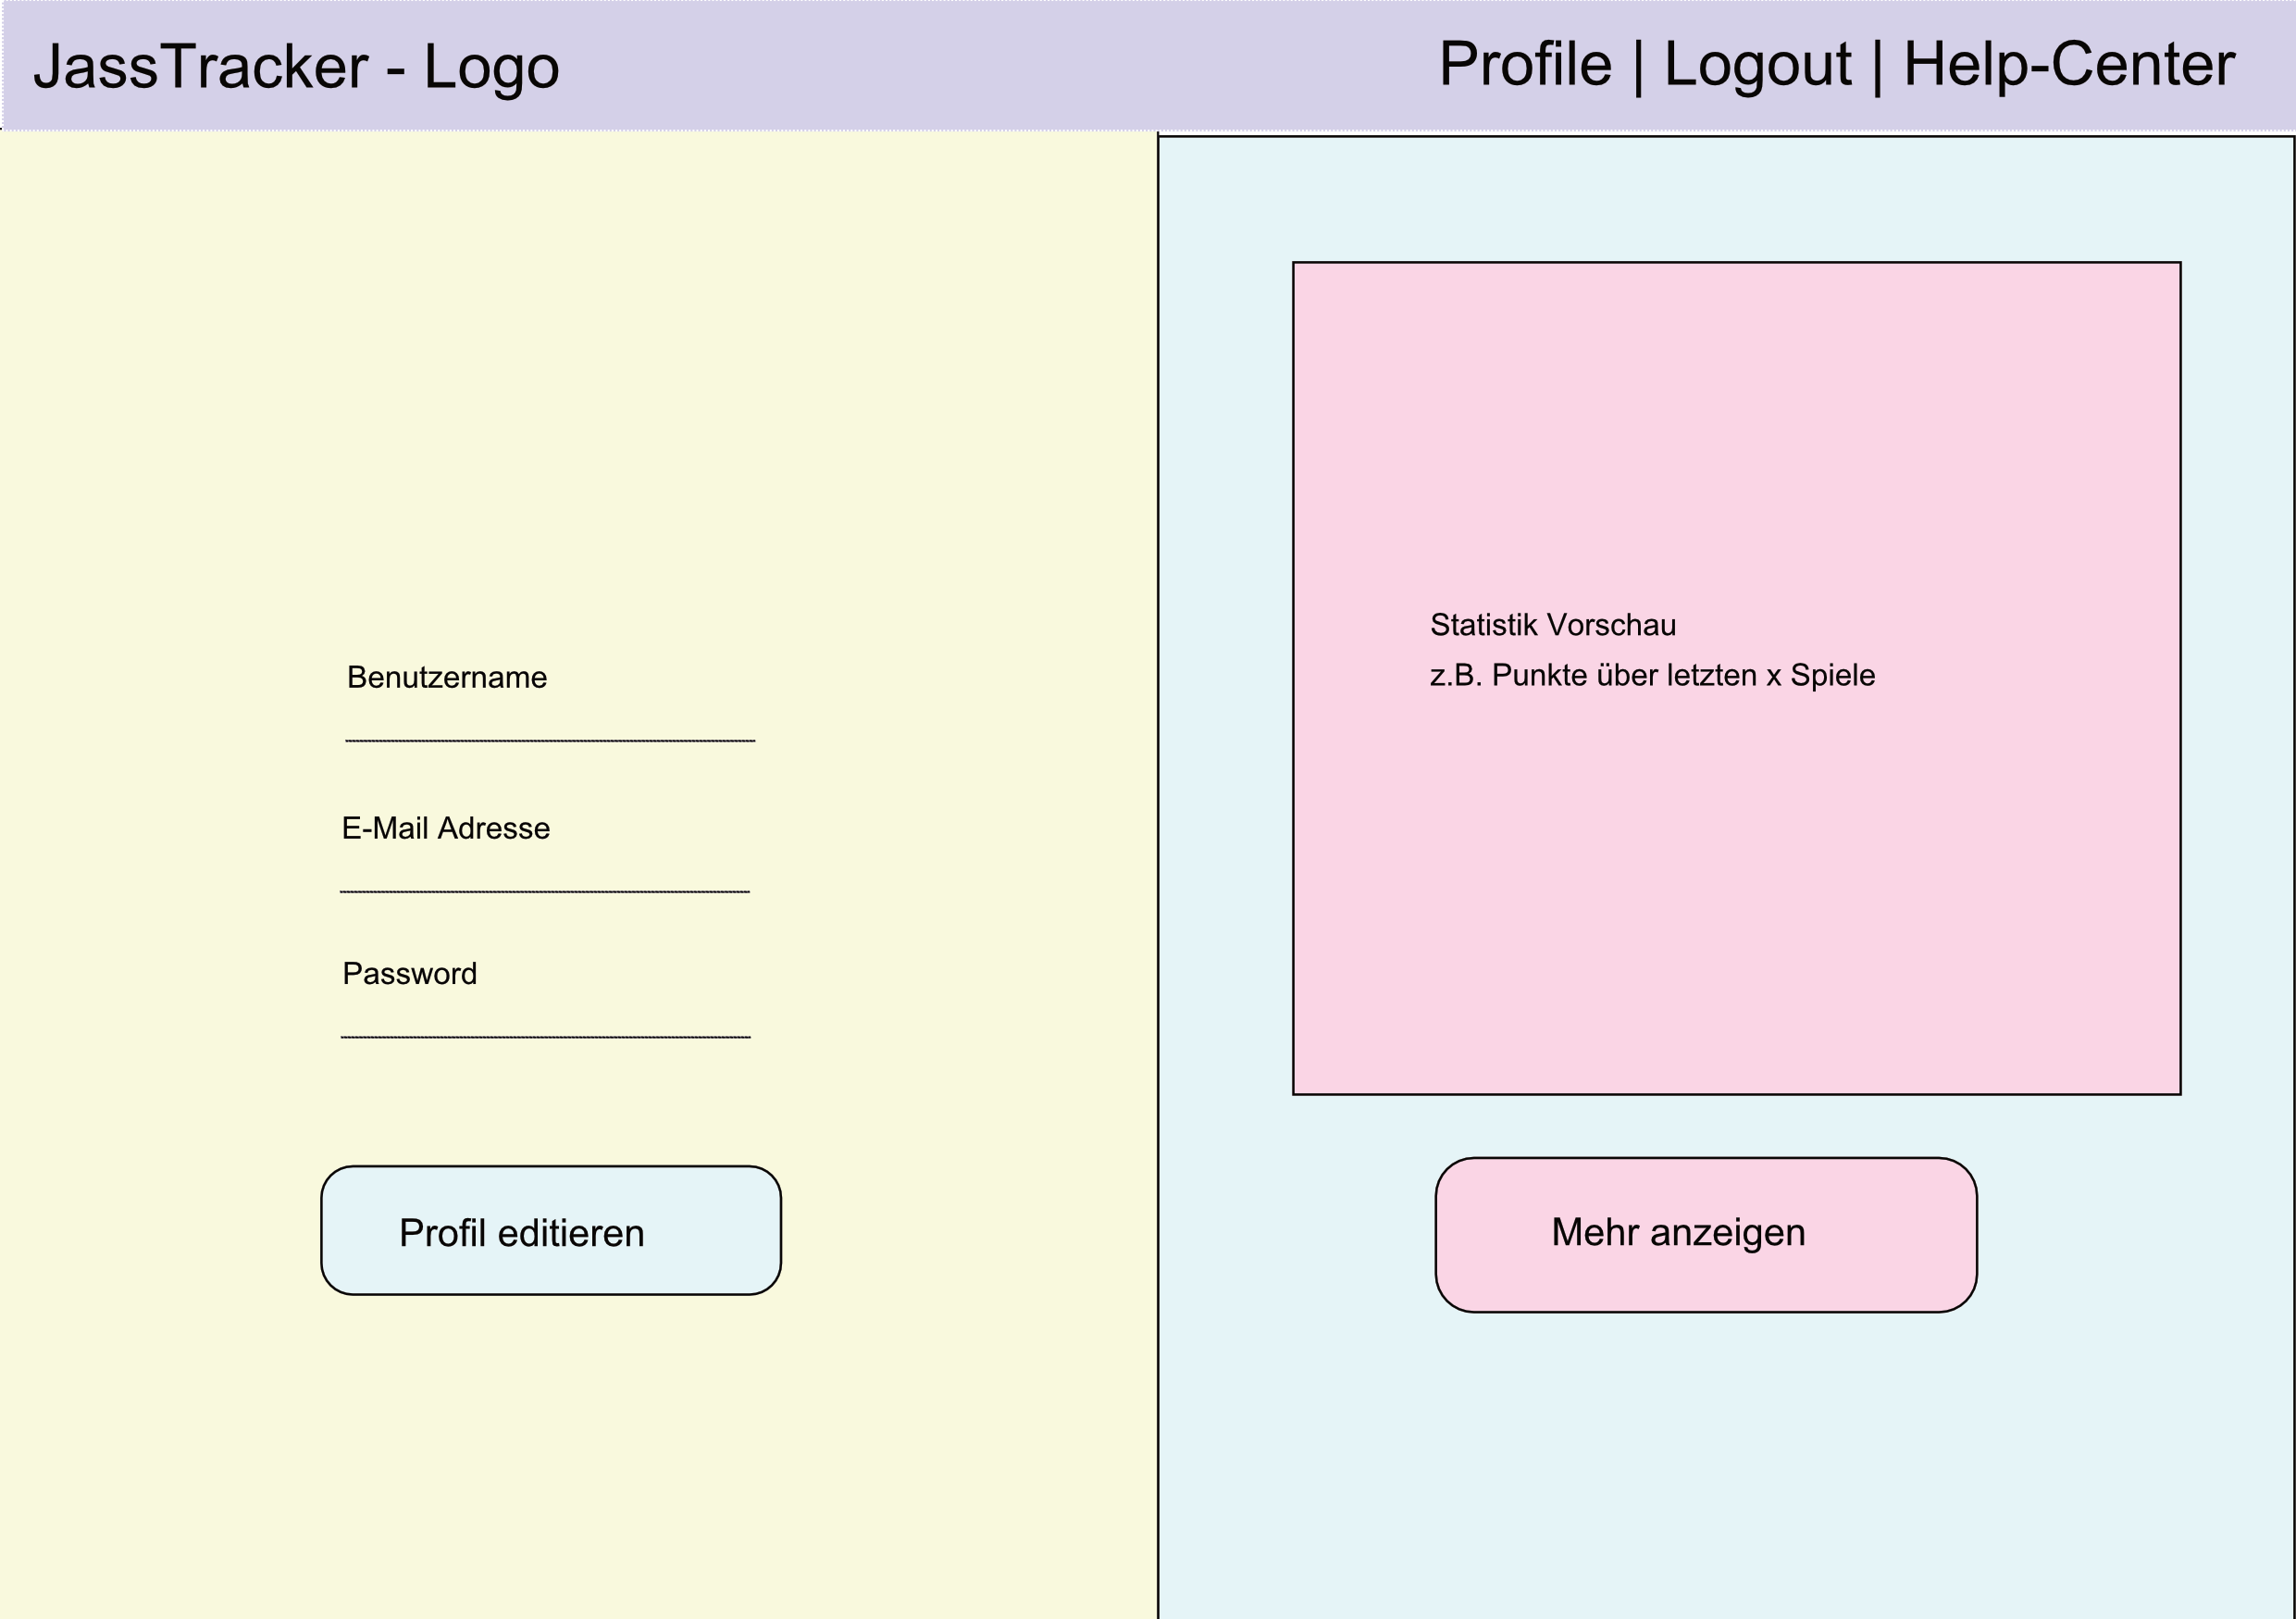
\includegraphics[height=10cm, width=\textwidth]{resources/mockups/mockup-profile-overview}
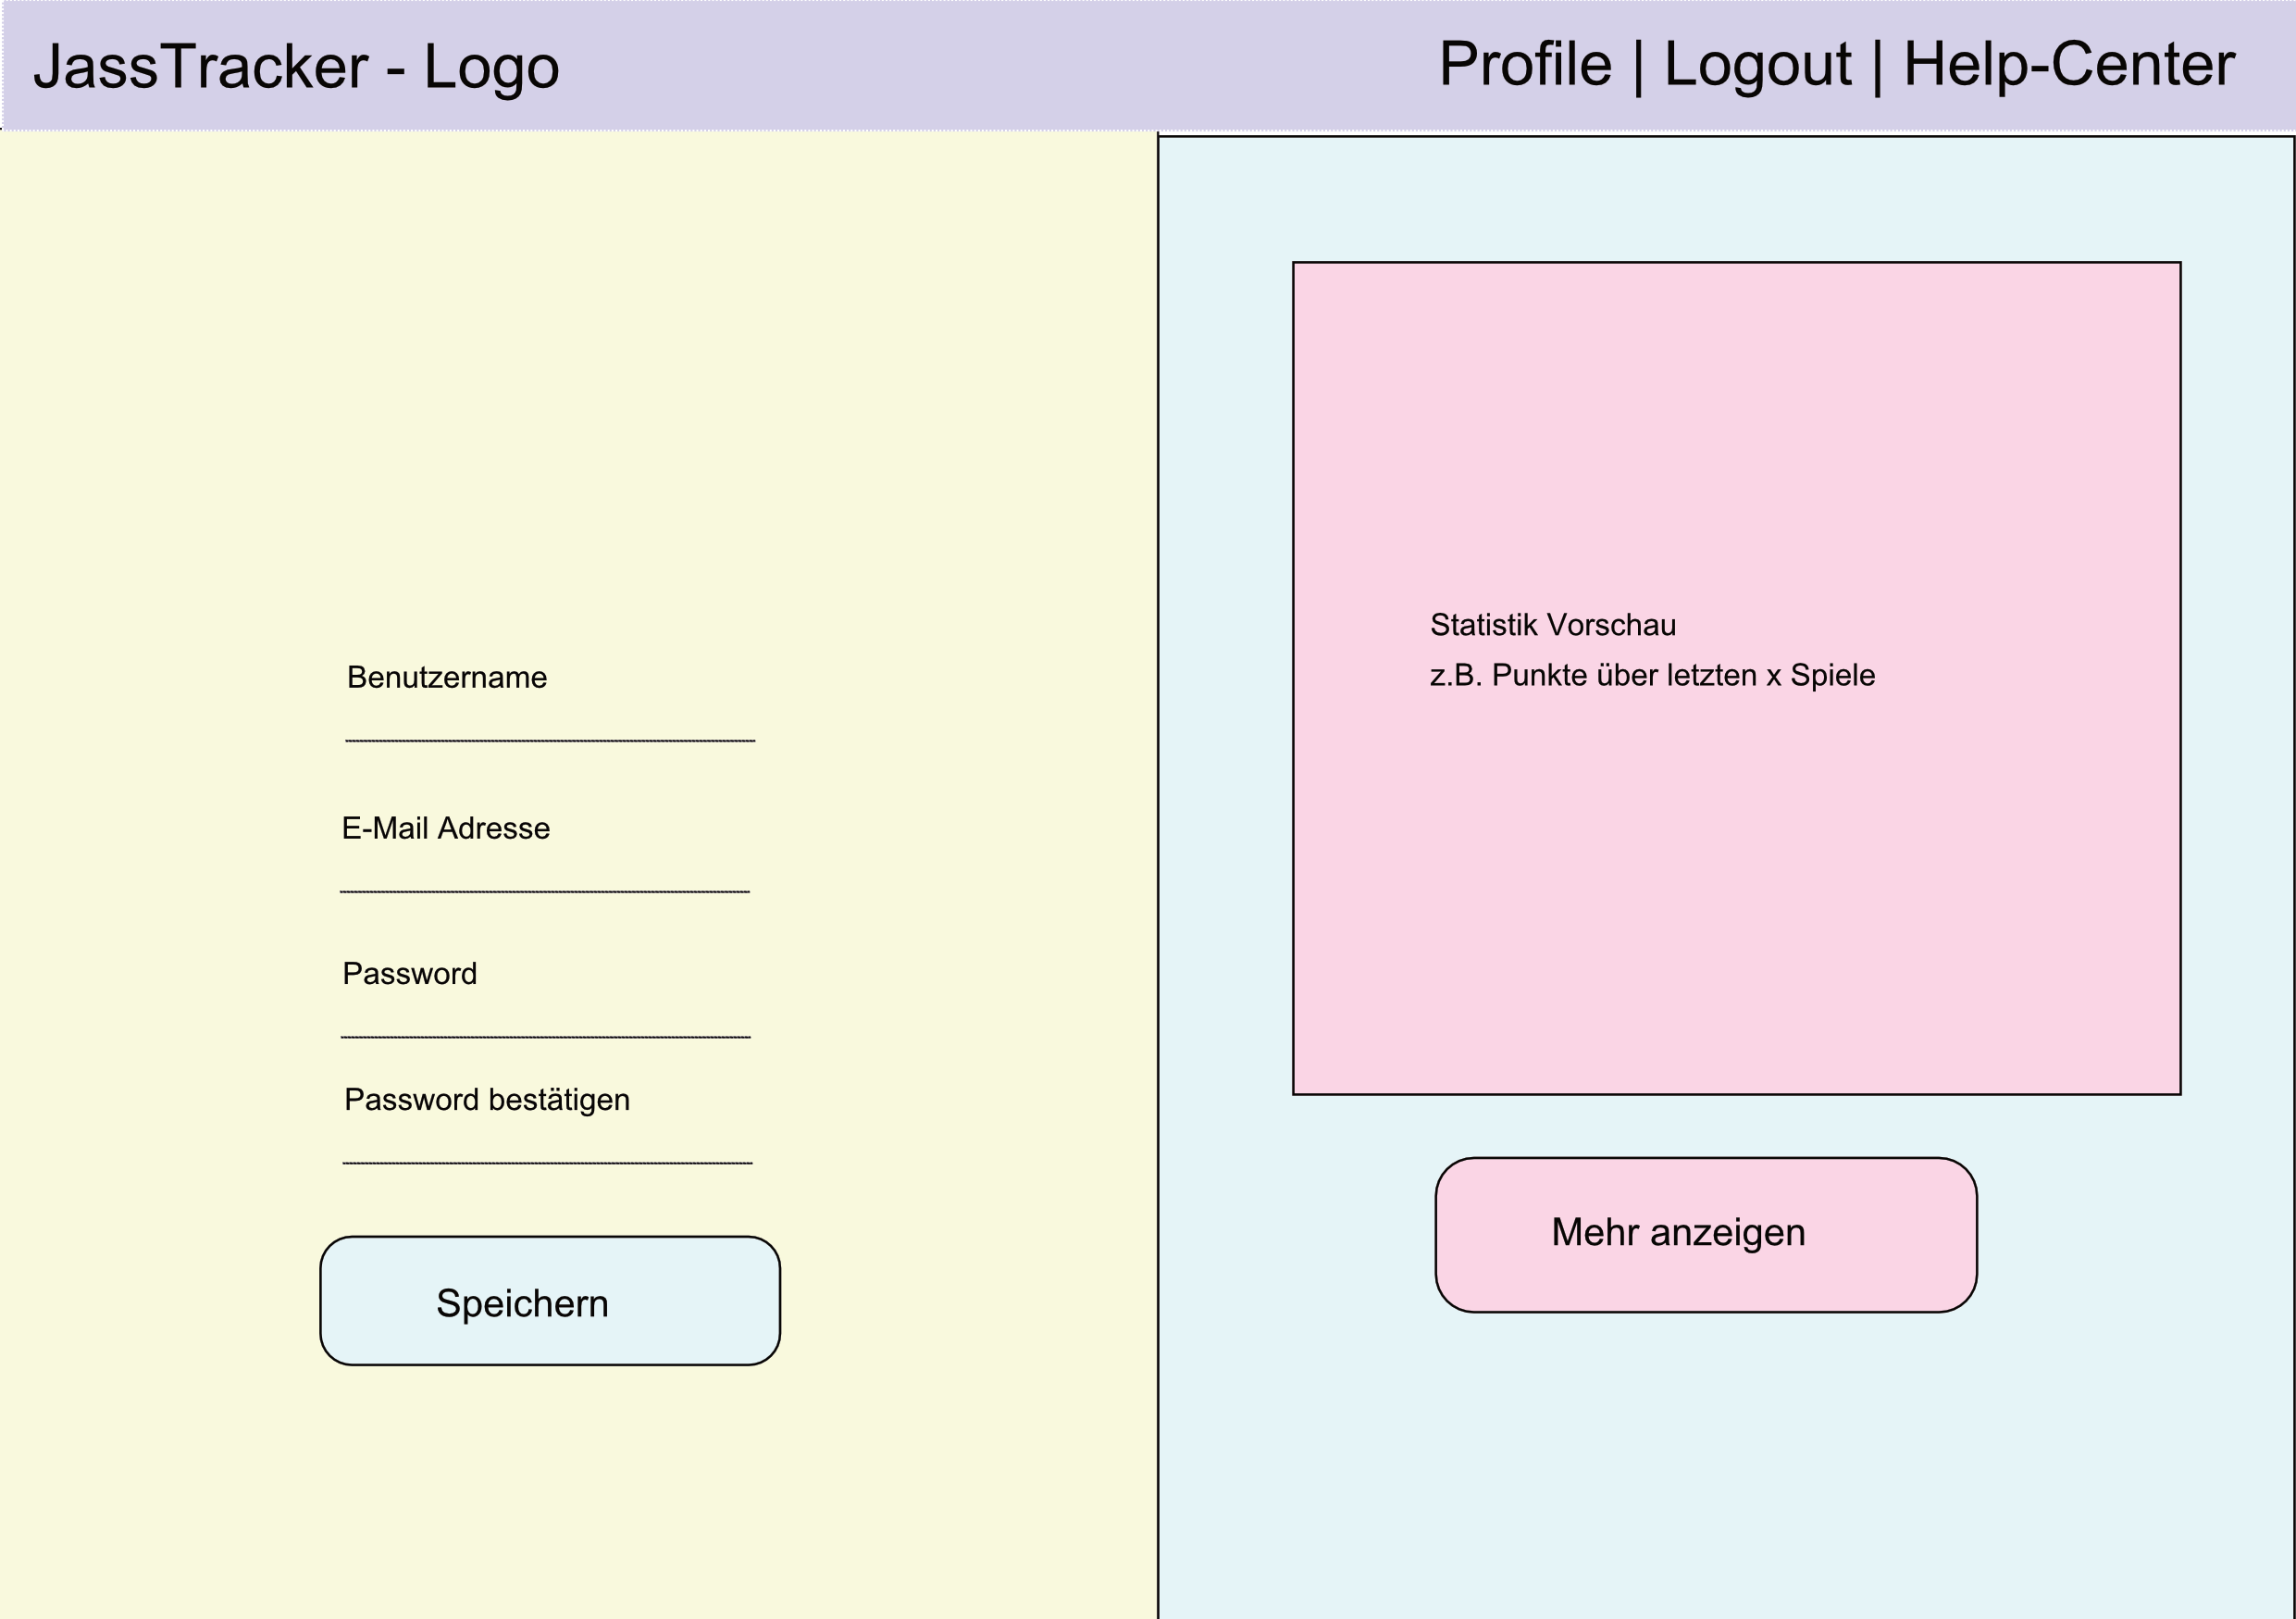
\includegraphics[height=10cm, width=\textwidth]{resources/mockups/mockup-profile-overview-edit}
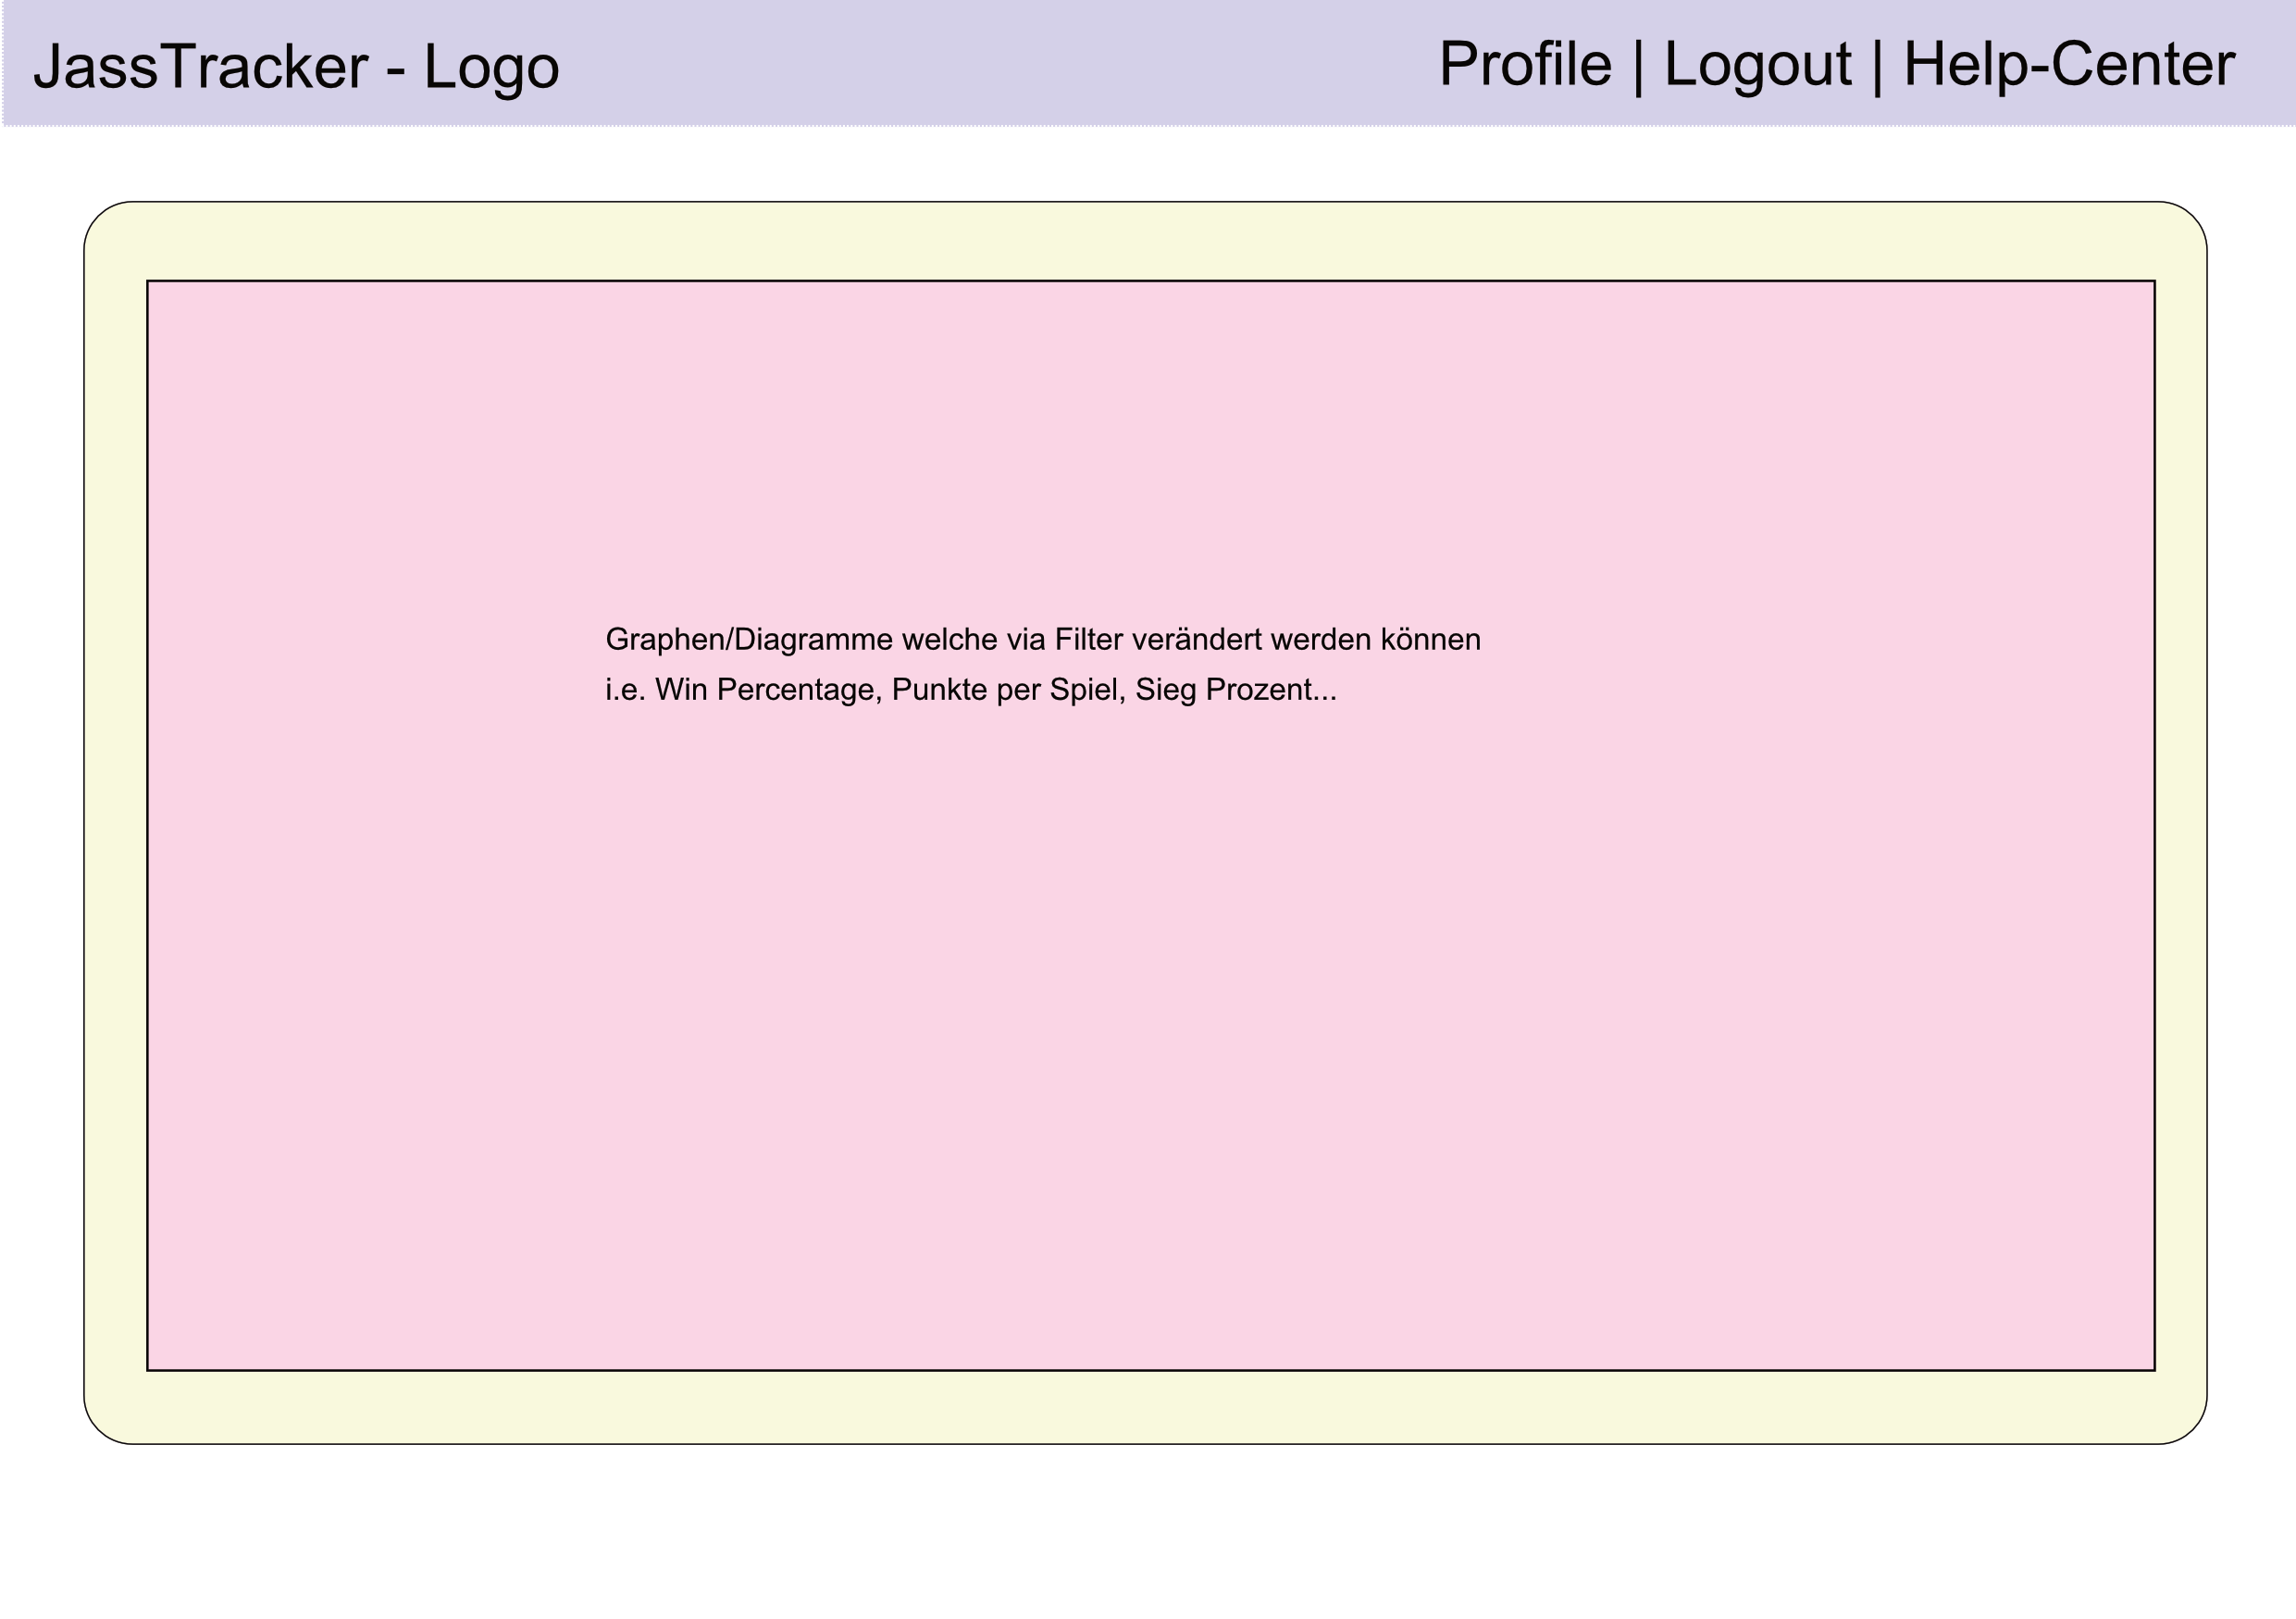
\includegraphics[height=10cm, width=\textwidth]{resources/mockups/mockup-player-stats}
